\documentclass[UTF8,zihao=-4,a4paper,fontset=none]{ctexart}
\usepackage[left=22mm,right=22mm,top=23mm,bottom=23mm,headheight=15pt]{geometry}
\usepackage{fontspec,anyfontsize}
\setmainfont{FZFSK.TTF}[Path=/usr/share/fonts/wps-office/,AutoFakeBold=2,AutoFakeSlant=0.15]
\setsansfont{FZFSK.TTF}[Path=/usr/share/fonts/wps-office/,AutoFakeBold=2,AutoFakeSlant=0.15]
\setmonofont{FZFSK.TTF}[Path=/usr/share/fonts/wps-office/,AutoFakeBold=2,AutoFakeSlant=0.15]
\setCJKmainfont{FZFSK.TTF}[Path=/usr/share/fonts/wps-office/,AutoFakeBold=2]
\setCJKsansfont{FZFSK.TTF}[Path=/usr/share/fonts/wps-office/,AutoFakeBold=2]
\setCJKmonofont{FZFSK.TTF}[Path=/usr/share/fonts/wps-office/,AutoFakeBold=2]
\newCJKfontfamily\coverfangsong{FZFSK.TTF}[Path=/usr/share/fonts/wps-office/]
\usepackage{graphicx,float,booktabs,tabularx,longtable,array,enumitem,xcolor,amsmath}
\usepackage[most]{tcolorbox}
\usepackage{caption,fancyhdr,hyperref,bookmark,lastpage,microtype}
\microtypesetup{protrusion=false}
\definecolor{forest}{HTML}{246349}
\definecolor{ink}{HTML}{20332A}
\definecolor{muted}{HTML}{627264}
\definecolor{soft}{HTML}{EEF3E9}
\hypersetup{unicode=true,colorlinks=true,linkcolor=forest,urlcolor=forest,citecolor=forest,pdftitle={校园集：校园二手交易系统——实验二软件设计与建模},pdfauthor={王天祥},pdfsubject={软件设计、UML建模与UI原型实验报告}}
\urlstyle{same}
\setlength{\parindent}{2em}
\setlength{\parskip}{3pt}
\linespread{1.22}
\setlist{nosep,leftmargin=2em,topsep=4pt,itemsep=3pt}
\setlist[itemize]{label=\(\bullet\)}
\renewcommand{\arraystretch}{1.25}
\setlength{\tabcolsep}{5pt}
\captionsetup{font=small,labelfont=bf,labelsep=quad,skip=7pt}
\ctexset{section={format=\Large\sffamily\bfseries\color{ink},beforeskip=18pt,afterskip=12pt},subsection={format=\large\sffamily\bfseries\color{ink},beforeskip=12pt,afterskip=8pt},subsubsection={format=\normalsize\sffamily\bfseries,beforeskip=8pt,afterskip=4pt}}
\pagestyle{fancy}
\fancyhf{}
\fancyhead[L]{\small\sffamily 校园集 · 软件设计与建模}
\fancyhead[R]{\small\sffamily 实验二}
\fancyfoot[C]{\small\thepage}
\renewcommand{\headrulewidth}{0.4pt}
\raggedbottom
\newcolumntype{Y}{>{\raggedright\arraybackslash}X}
\newtcolorbox{keypoint}{colback=soft,colframe=soft,boxrule=0pt,arc=2mm,left=4mm,right=4mm,top=2mm,bottom=2mm,fontupper=\small}
\begin{document}
\begin{titlepage}
\thispagestyle{empty}
\vspace*{15mm}
\begingroup
\centering
\coverfangsong
{\fontsize{28}{42}\selectfont 软件工程}\par
\vspace{10mm}
{\fontsize{18}{28}\selectfont 实验二：软件设计与建模}\par
\vspace{8mm}
{\fontsize{18}{28}\selectfont 二手交易系统}\par
\endgroup
\vspace{8mm}
\noindent{\color{forest}\rule{\textwidth}{1.2pt}}\par
\vspace{12mm}
\begin{tabular}{@{}ll}
\textbf{姓名} & 王天祥\\[8pt]
\textbf{学号} & 241220095\\[8pt]
\textbf{日期} & 2026 年 11 月 9 日\\[8pt]
\textbf{材料范围} & UML 建模、界面原型与辅助工具记录
\end{tabular}
\vfill
\begin{keypoint}
\textbf{版本说明：实验二设计报告。}\par
本报告根据实验一最终需求、现有 PlantUML 源文件和 UI 截图编排，
辅助工具的使用范围与设计取舍见第4章。界面数据为模拟数据，
不代表已实现或已通过真实系统验收。
\end{keypoint}
\end{titlepage}
\pagenumbering{Roman}
\setcounter{tocdepth}{2}
\begingroup
\small\linespread{1.0}\selectfont
\tableofcontents
\endgroup
\clearpage
\pagenumbering{arabic}
\section{软件的主要功能}
\subsection{项目定位与功能范围}
校园集面向校内闲置物品交易，围绕“商品发布、平台审核、买家预约、卖家确认、线下交付、买家确认完成”组织业务。
每条商品记录对应一件独立物品，线上系统保存信息和交易意向状态，付款、验货和交付在线下完成。
系统不接入真实支付、退款、物流、即时聊天、竞价或推荐算法，也不开发独立手机应用。


普通用户可以在不同交易中分别作为买家和卖家，不需要注册两套账户，但不能预约本人商品。
管理员负责审核、违规处置、终止申请核实、日志与统计查询，不能擅自改写卖家价格或代买家确认完成。
游客仅能浏览已发布商品的公开信息。

本地预览时，双击相应 HTML 文件，用浏览器打开即可。

\subsection{功能模块划分}
\begin{table}[H]\centering\small
\caption{功能模块与职责}
\begin{tabularx}{\linewidth}{@{}p{32mm}Y@{}}\toprule
模块 & 主要职责\\\midrule
账户与权限 & 注册登录、角色和资源归属校验、联系方式访问控制\\
商品管理 & 保存草稿、送审撤回、修改、普通下架及重新送审\\
审核与违规处置 & 审核决定及历史、违规原因与限制、普通终止审批\\
商品查询与展示 & 多条件查询、排序、分页、公开详情及可见范围\\
预约与交易 & 请求幂等、交易快照、预约状态、取消、确认、超时、完成和终止\\
通知 & 登记待发送消息、提交后投递、重试与已读管理\\
分类与交易统计 & 商品数量、分类状态分组、完成笔数与快照金额\\
操作日志 & 记录关键成功与失败操作，提供只读组合查询\\\bottomrule
\end{tabularx}
\end{table}

数据持久化是上述模块共用的支撑组件，保存用户、商品、预约、请求结果、审核及终止记录、通知和日志，承担关联、唯一性与原子提交的保障。
该划分是同一应用中的逻辑模块划分，并不表示每个模块都独立部署为微服务。


\clearpage

\subsection{业务规则与质量约束}
\begin{enumerate}
\item \textbf{审核后发布。} 草稿可缺项，送审须校验标题、描述、分类、价格、图片和交付地点。
已发布商品修改业务字段时同步停止公开并转待审核；有效预约期间不允许改价或普通下架。
\item \textbf{商品与预约分开维护状态。} 商品“已预约”对应预约“待卖家确认”，商品“已确认”对应预约“已确认”。历史预约可以多条，有效预约同一时刻最多一条。
\item \textbf{旧页面与重复请求分别处理。} 新动作须验证当前状态、版本与价格；同一买家的同请求标识重试返回原结果，并附关联预约当前状态。
\item \textbf{终止区分业务依据。} 确认后的普通终止必须经管理员核实双方同意，商品转普通已下架；违规处置可以直接终止有效预约，商品转违规下架。
\item \textbf{历史不得反向改写。} 交易完成后再发现违规，只追加记录并隐藏商品，商品和预约仍为已完成；快照和历史记录保留。
\end{enumerate}


关键变更须把商品、预约、处理记录、成功日志及通知待发送记录作为一次整体提交。
任何必要写入失败都不能留下半成功状态；实际通知发送在提交后执行，发送失败不回滚已提交业务。
数据库唯一约束作为并发兜底，不能仅依靠前端隐藏按钮。

\begin{table}[H]\centering\small
\caption{非功能要求及本阶段边界}
\begin{tabularx}{\linewidth}{@{}p{29mm}Y@{}}\toprule
类别 & 设计约束\\\midrule
查询与预约性能 & 固定环境和数据集下评估查询及并发预约响应；同商品最多一条有效预约。原型未开展真实负载验收。\\
凭据与隐私 & 密码使用独立随机盐和适合密码用途的哈希；联系方式不进入公开列表、详情和日志。\\
持久性与恢复 & 已提交业务在应用重启后保持；成功备份间隔不超过24小时，保留最近7份；整库恢复目标30分钟、数据丢失窗口不超过24小时。\\
可用性与适配 & 核心页面应兼顾桌面与手机浏览器，具体用户任务用时及适配指标须后续独立验收。\\\bottomrule
\end{tabularx}
\end{table}


\begin{keypoint}
本阶段交付的是设计与静态交互原型。界面上的商品数量、交易金额、处理状态和通知均为演示数据；前端校验不替代服务端鉴权、事务、并发约束、备份或性能验证。
\end{keypoint}


\clearpage

\section{软件架构 UML 设计}
\subsection{结构性图：组件图}
组件图展示八个业务模块、公共能力以及数据持久化组件。依赖箭头由使用方指向被依赖方，包级箭头汇总同类依赖；它们不表示调用发生的时间顺序。



\begin{figure}[H]
\centering
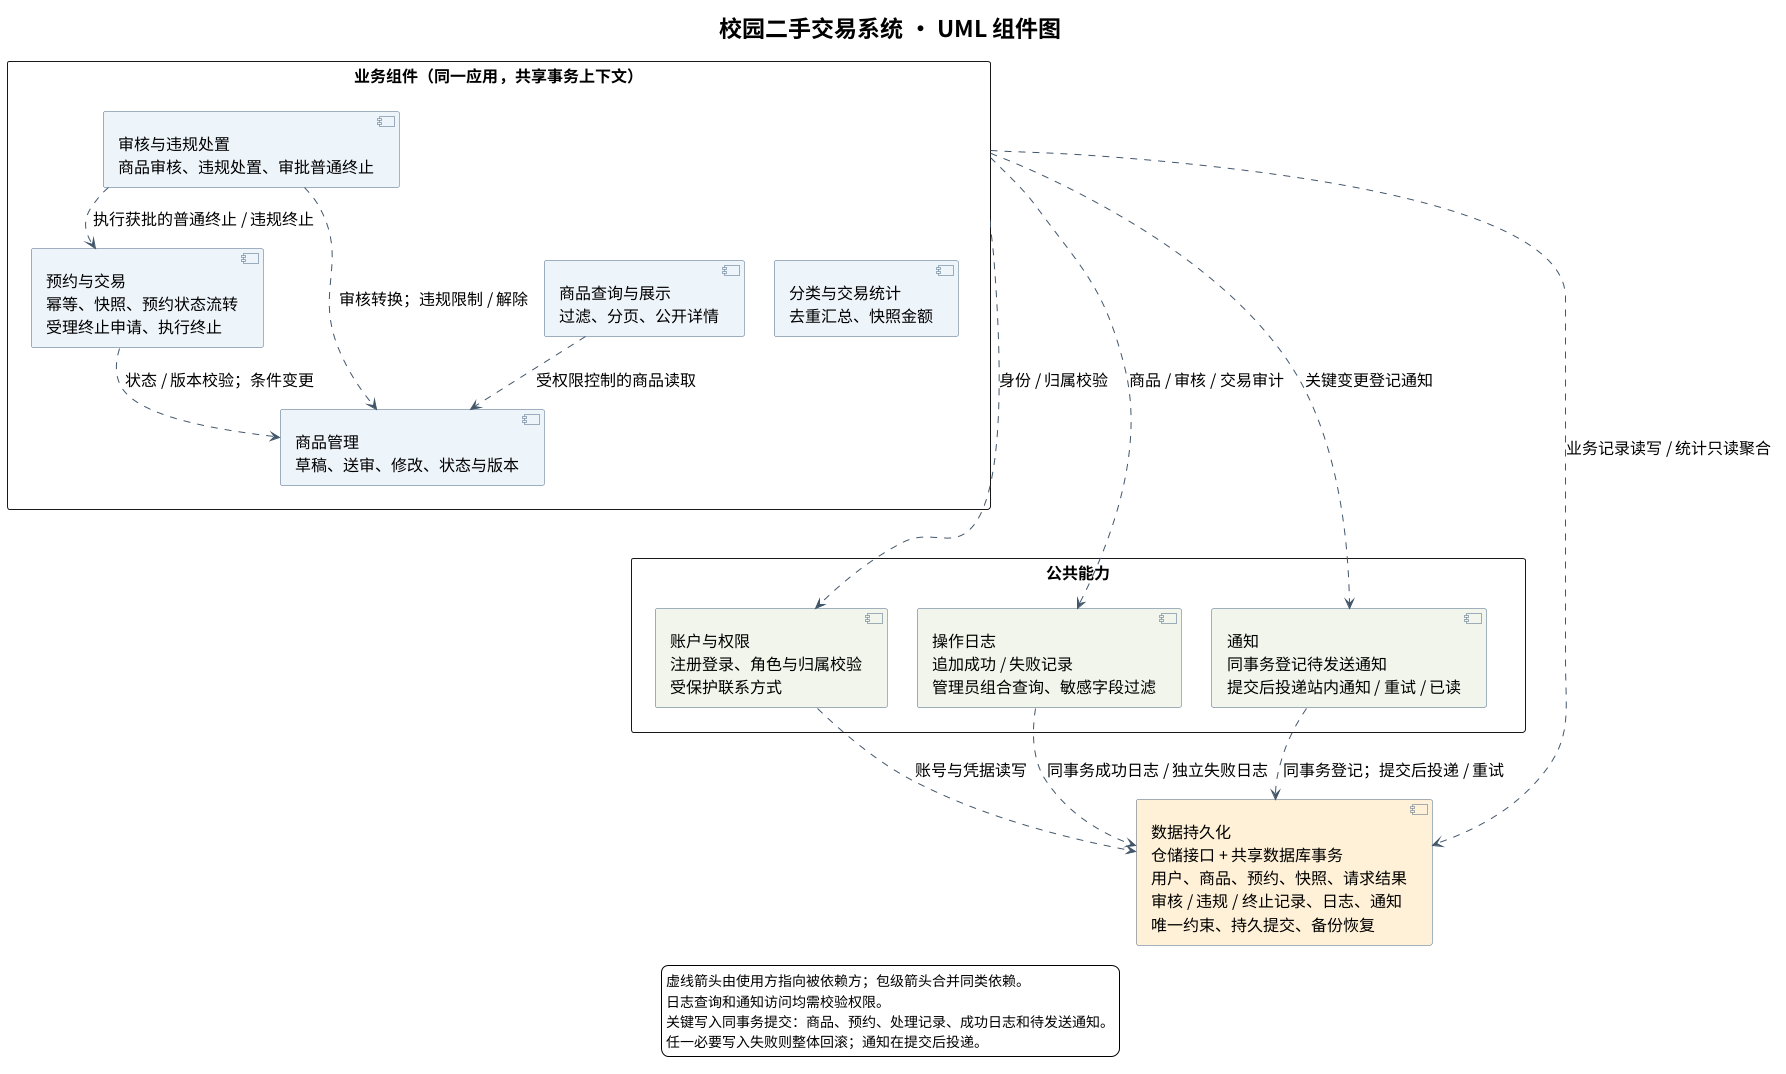
\includegraphics[width=\linewidth,height=0.46\textheight,keepaspectratio]{UML/组件图.png}
\caption{系统组件与关键依赖（结构性图）}
\end{figure}


预约与交易模块通过商品管理接口校验状态、版本和可售条件，避免在不同用例中分散修改商品状态。
审核与违规处置模块调用预约与交易执行获批的普通终止或违规终止，并调用商品管理执行审核或销售限制。
日志与通知作为公共能力参与关键业务提交。

共享数据库事务使跨商品、预约和审计记录的更新保持原子性，适合课程项目的单实例规模。
通知的“登记”和“投递”分离，避免外部发送失败迫使已经成功的预约回滚。
查询和统计读取已提交数据，统计不在每次重试时简单增加计数。




\clearpage

\subsection{结构性图：领域类图}
领域模型以 \texttt{User}、\texttt{Product} 和 \texttt{Reservation} 为核心，辅以请求记录、审核、终止申请、违规处置、通知及操作日志。
图中买家和卖家使用关联角色表达，不建立两种互斥的用户子类。



\begin{figure}[H]
\centering
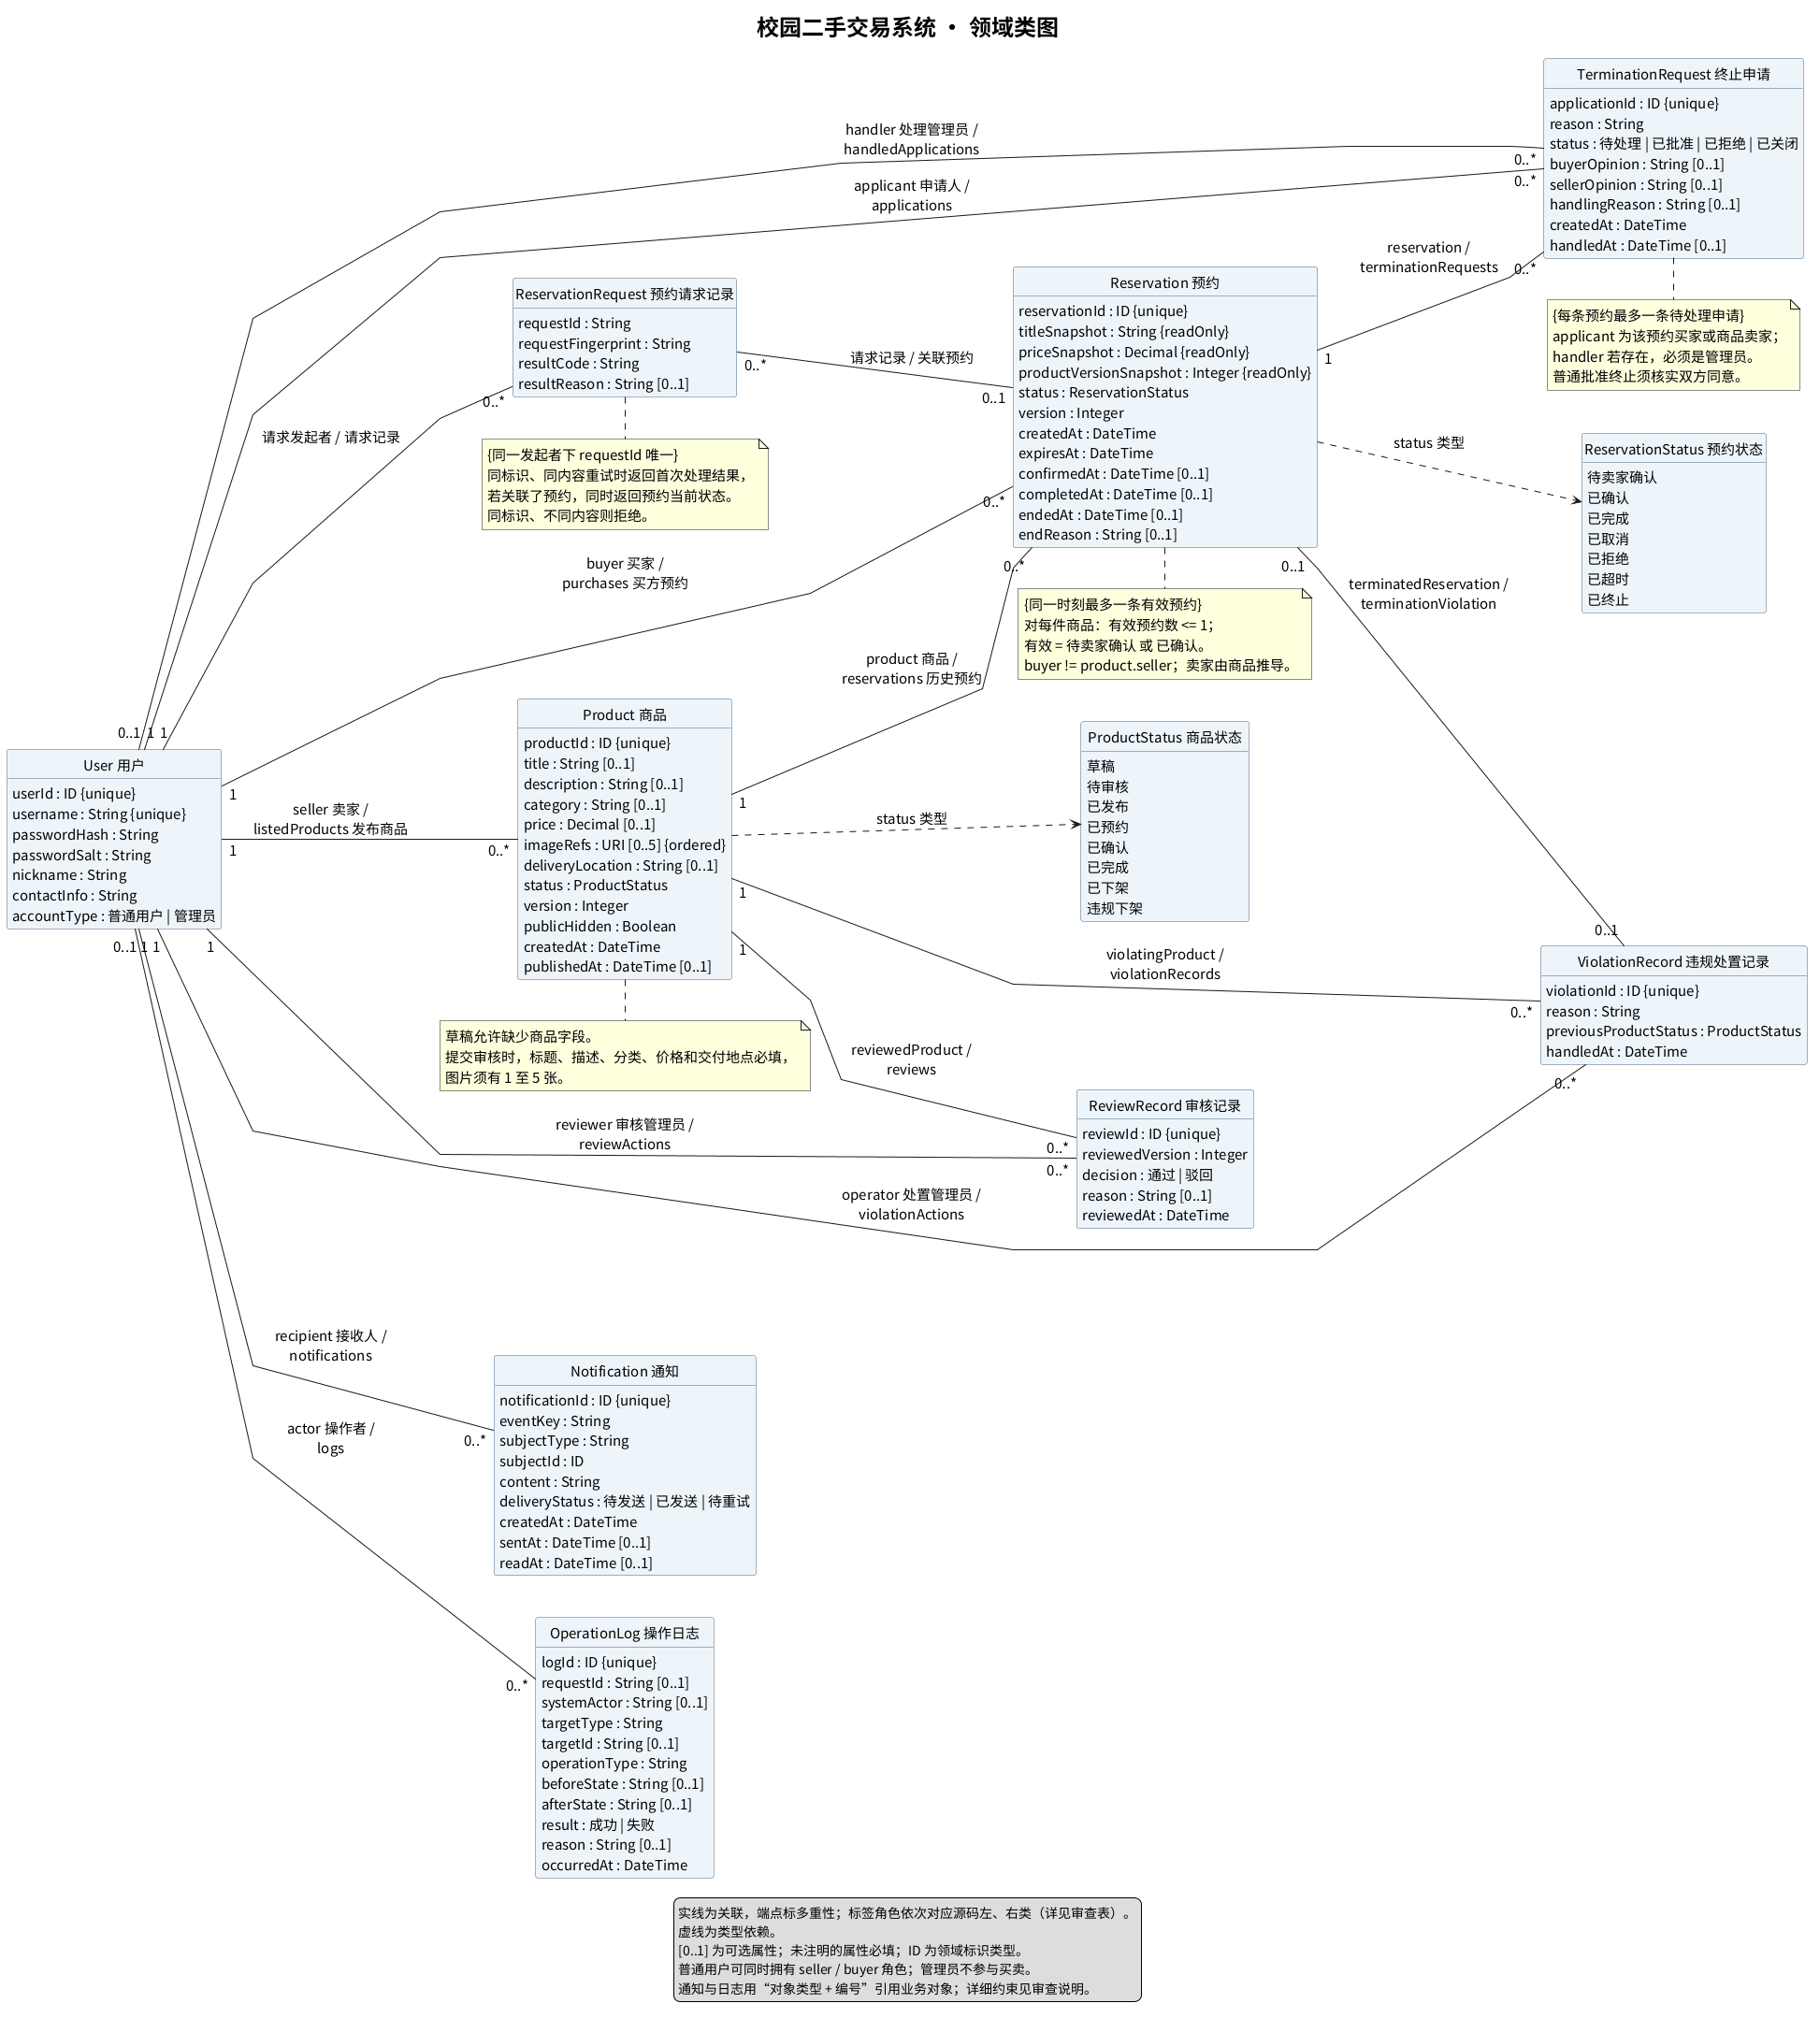
\includegraphics[width=\linewidth,height=0.72\textheight,keepaspectratio]{UML/类图.png}
\caption{领域类、属性及关联总览（结构性图；细节可放大原图查看）}
\end{figure}


\noindent\small 核心数据关系和约束见下一页。

\clearpage

\subsubsection{关联与多重性}
\begin{table}[H]\centering\small
\caption{核心领域关联的含义}
\begin{tabularx}{\linewidth}{@{}p{49mm}Y@{}}\toprule
关联 & 含义\\\midrule
User--Product & 每件商品有一位 \texttt{seller}，一个用户可发布0至多件商品。\\
User--Reservation & 每条预约有一位 \texttt{buyer}，一个用户可发起0至多条预约。\\
Product--Reservation & 每条预约对应一件商品，商品可保留0至多条历史预约；不能将历史多重性误写为0至1。\\
User--ReservationRequest & 同一发起者下 \texttt{requestId} 唯一；多条请求记录可以关联同一预约，请求失败时也可无关联预约。\\
Product--ReviewRecord & 每件商品可有多次审核记录，每条记录关联审核管理员及被审核版本。\\
Reservation--TerminationRequest & 预约可有历史终止申请，同一时刻最多一条待处理申请；申请人为参与者。\\
Product--ViolationRecord & 保存针对商品的历史违规处置，记录原因、管理员和时间。\\
User--Notification / OperationLog & 通知对应一个接收人；日志操作者可以是用户或系统身份。\\\bottomrule
\end{tabularx}
\end{table}
\subsubsection{数据约束与建模选择}
\begin{itemize}
\item \textbf{有效预约唯一。} 对每件商品，状态属于待卖家确认或已确认的预约数不得超过1；历史终态记录完整保留。
\item \textbf{禁止自购。} \texttt{reservation.buyer} 不得等于 \texttt{reservation.product.seller}。
\item \textbf{快照不可反向覆盖。} 预约保存标题、价格和商品版本快照，后续修改商品不能改变原交易约定。
\item \textbf{状态与可见性分离。} \texttt{publicHidden} 支持已完成商品事后违规隐藏，不把完成状态改为违规下架。
\item \textbf{请求与预约分离。} \texttt{ReservationRequest} 保存内容指纹和首次结果，以覆盖失败重放、新请求返回已有预约等情形。
\end{itemize}

审核记录仅表示已作出的通过或驳回决定；提交和撤回由商品状态及操作日志体现。
普通终止的双方意见及处理结果暂保存在终止申请内，违规终止另有违规记录。
通知和日志用对象类型及编号引用目标，这一逻辑引用形式仍需在实现阶段落实关联检查。



\clearpage

\subsection{行为性图：商品状态图}
商品维护草稿、待审核、已发布、已预约、已确认、已完成、已下架和违规下架八种状态。
“未完成商品”只是图中的复合分组，不是新增状态值。



\begin{figure}[H]
\centering
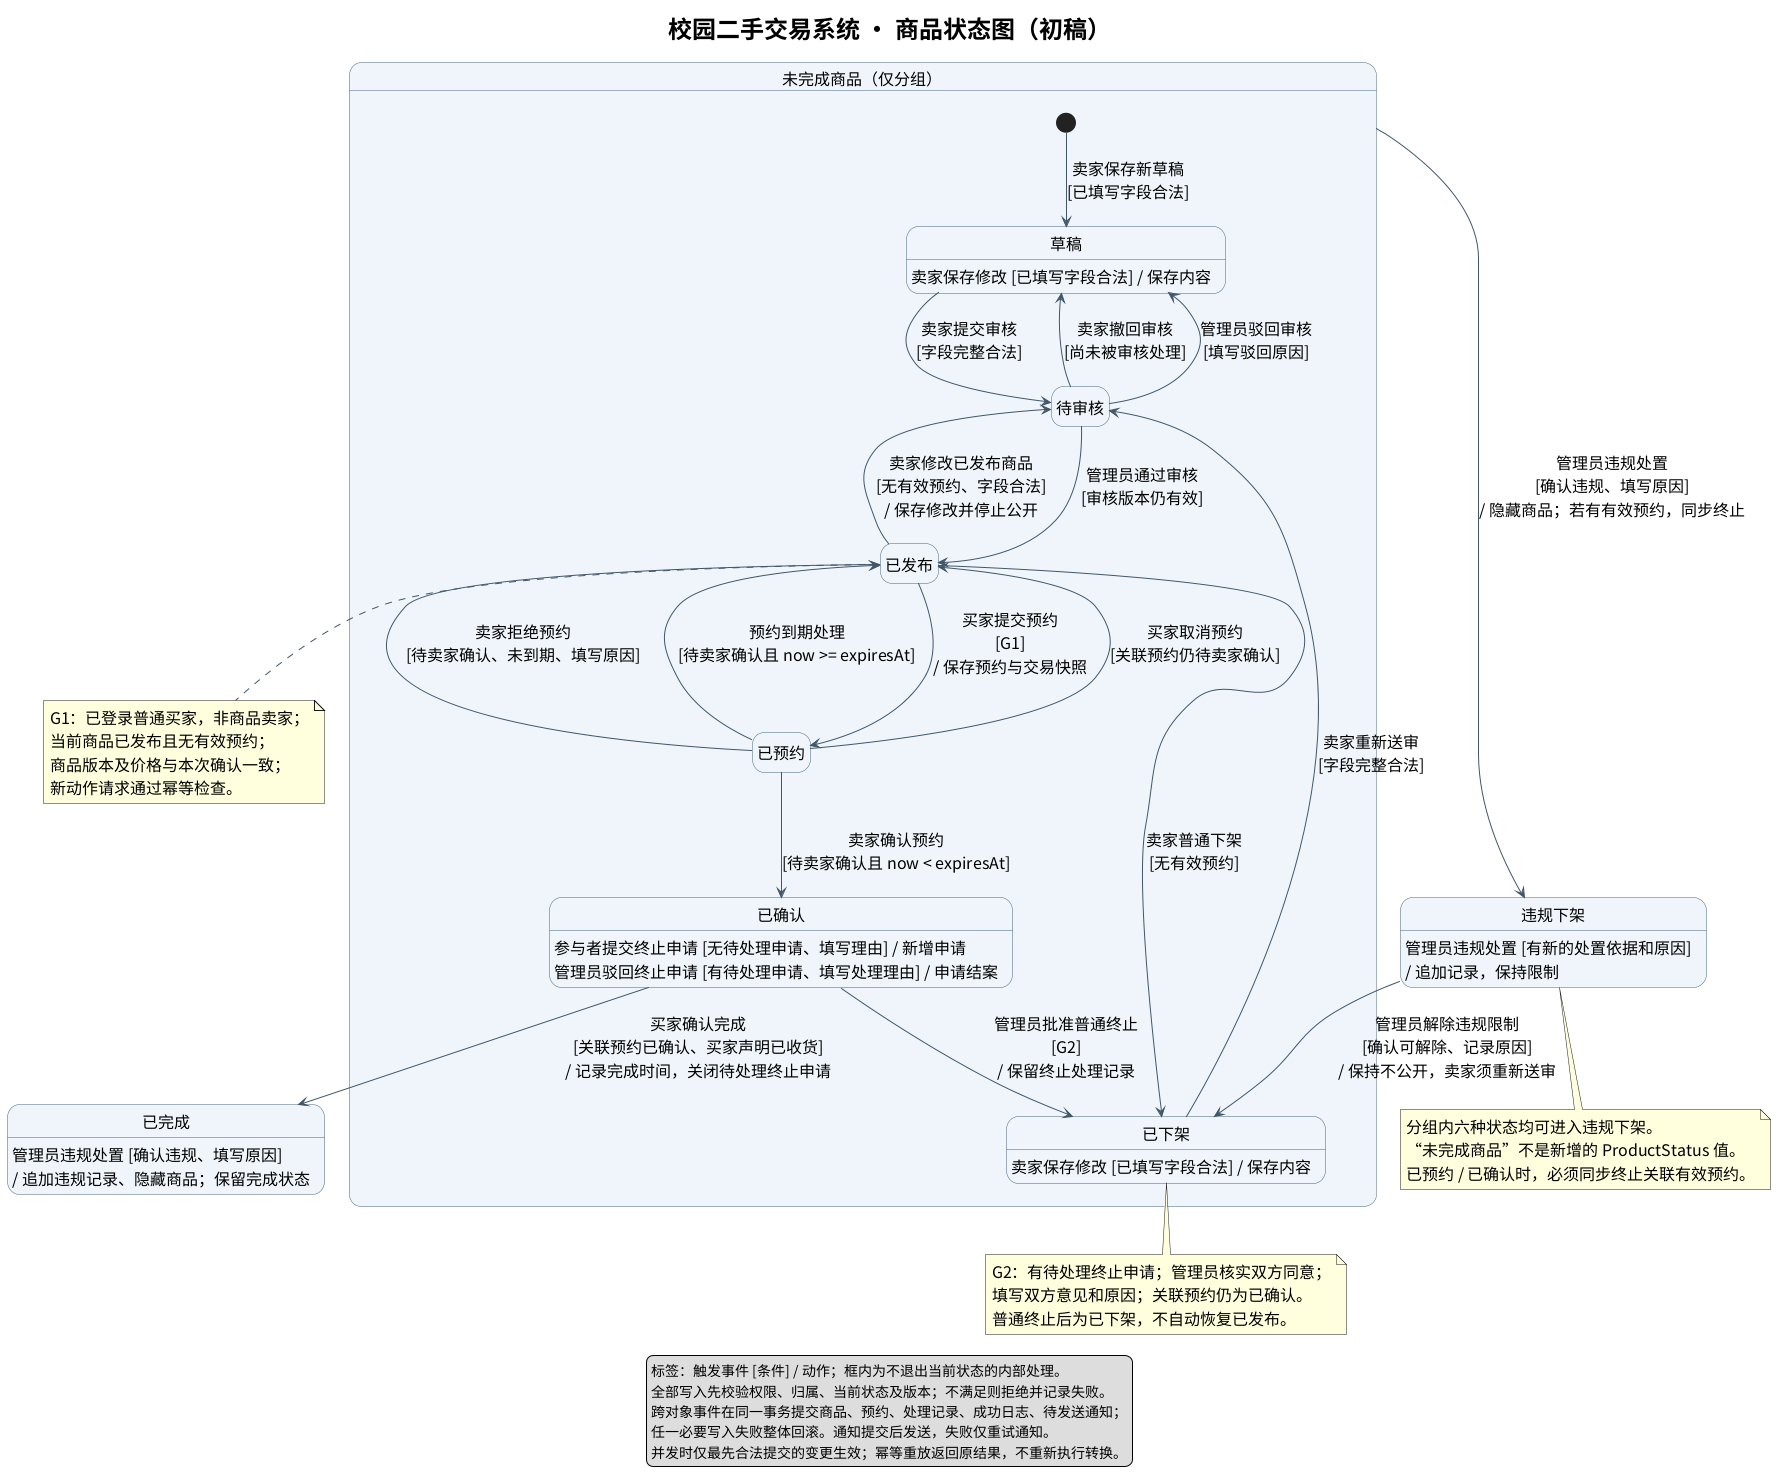
\includegraphics[width=\linewidth,height=0.59\textheight,keepaspectratio]{UML/商品状态图.png}
\caption{商品生命周期与违规例外（行为性图）}
\end{figure}


主线从草稿送审，经管理员通过后发布，再由预约、卖家确认和买家完成逐步推进。
取消、拒绝、超时仅能从已预约恢复已发布；确认后的普通终止转普通已下架，不立即复售。
违规限制解除后也只回普通已下架，仍需重新送审。

已完成状态内的违规事件只追加记录并隐藏商品，避免以状态回退破坏既有成交历史。
卖家不能通过修改或普通下架绕过有效预约约束。



\clearpage

\subsection{行为性图：预约状态图}
预约维护待卖家确认、已确认、已完成、已取消、已拒绝、已超时和已终止七种状态。
前两项是有效预约，其余是业务终态；需要再次预约时建立新记录，不能复活旧预约。



\begin{figure}[H]
\centering
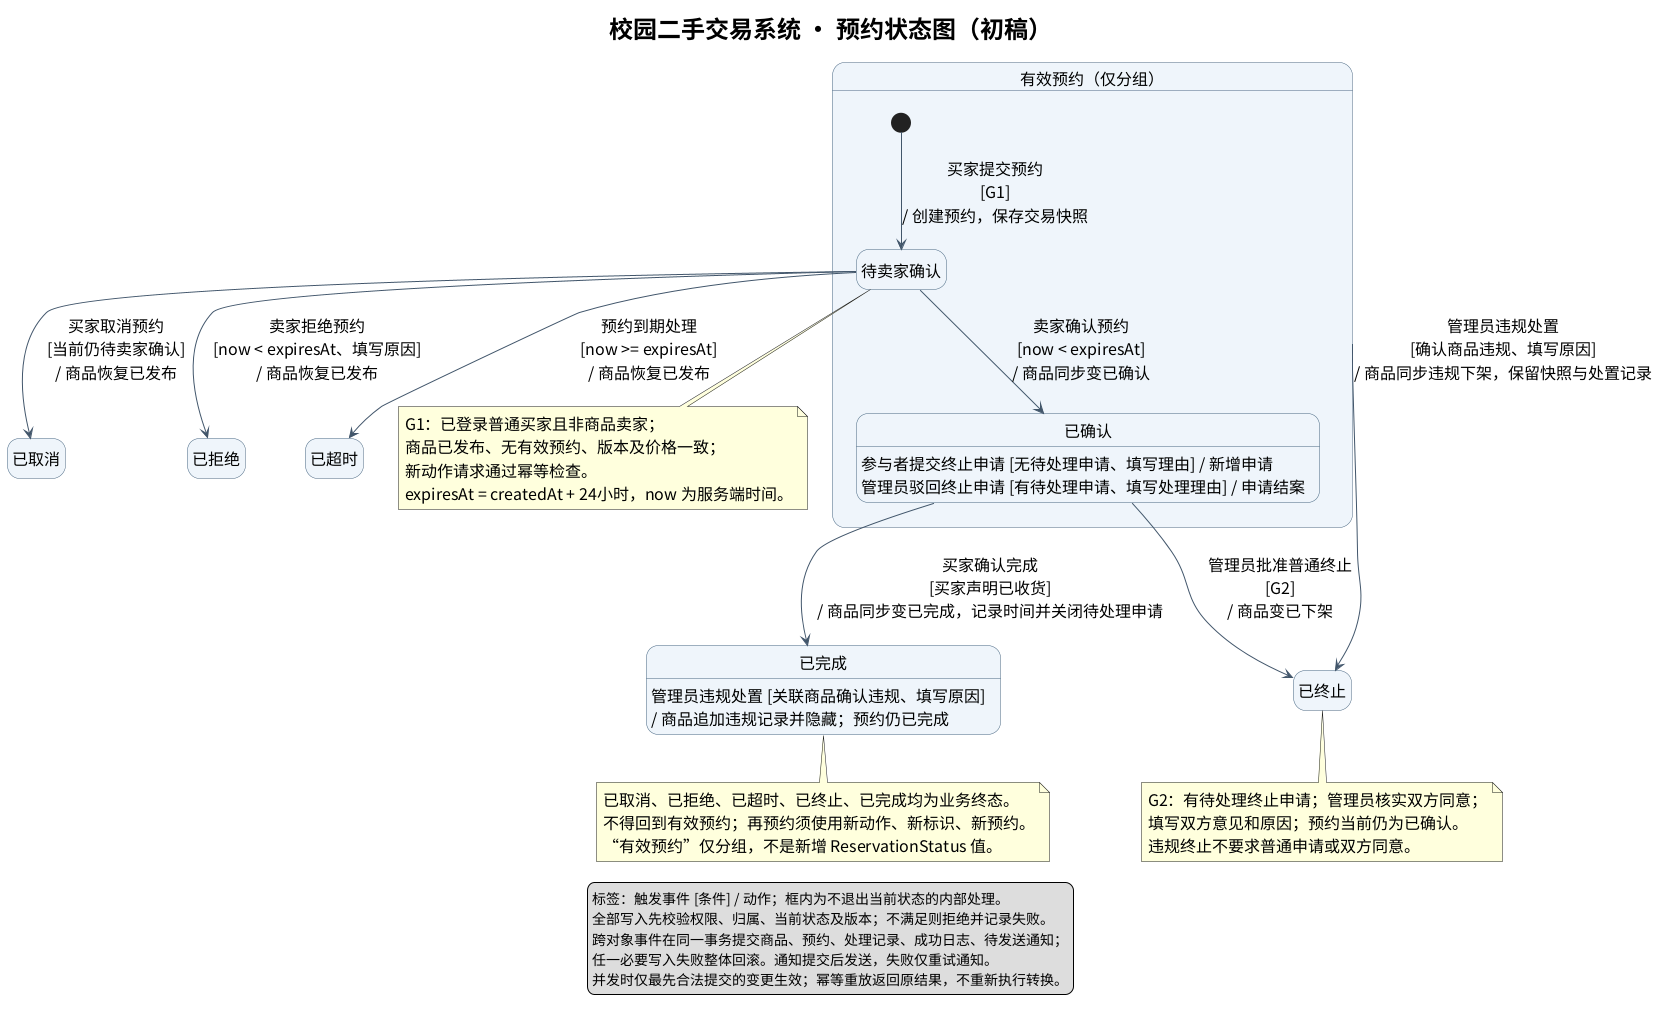
\includegraphics[width=\linewidth,height=0.43\textheight,keepaspectratio]{UML/预约状态图.png}
\caption{预约状态、普通终止与违规终止（行为性图）}
\end{figure}


卖家应在预约创建后24小时内确认或拒绝；拒绝须填写原因，到达截止时刻后不再接受确认或拒绝。
时间比较使用服务端时间，达到截止时刻即关闭确认与拒绝操作。

参与者提交终止申请、管理员驳回申请不会直接改变已确认状态。
普通终止须核实双方同意；违规终止不以普通申请或双方同意为条件。
买家完成交易时同时关闭待处理终止申请，防止此后继续终止。



\clearpage

\subsubsection{两套状态的联动与提交边界}
\begin{table}[H]\centering\small
\caption{跨商品与预约的统一事件}
\begin{tabularx}{\linewidth}{@{}p{34mm}Y Y@{}}\toprule
事件 & 商品结果 & 预约结果\\\midrule
买家提交预约 & 已发布 $\rightarrow$ 已预约 & 创建为待卖家确认\\
卖家确认预约 & 已预约 $\rightarrow$ 已确认 & 待卖家确认 $\rightarrow$ 已确认\\
买家取消预约 & 已预约 $\rightarrow$ 已发布 & 待卖家确认 $\rightarrow$ 已取消\\
卖家拒绝预约 & 已预约 $\rightarrow$ 已发布 & 待卖家确认 $\rightarrow$ 已拒绝\\
预约到期处理 & 已预约 $\rightarrow$ 已发布 & 待卖家确认 $\rightarrow$ 已超时\\
买家确认完成 & 已确认 $\rightarrow$ 已完成 & 已确认 $\rightarrow$ 已完成\\
管理员批准普通终止 & 已确认 $\rightarrow$ 已下架 & 已确认 $\rightarrow$ 已终止\\
管理员违规处置 & 未完成商品 $\rightarrow$ 违规下架 & 有效预约 $\rightarrow$ 已终止\\
完成后的违规处置 & 保持已完成，隐藏公开内容 & 保持已完成\\\bottomrule
\end{tabularx}
\end{table}

管理员违规下架时，先核对管理员身份、目标商品和最新业务状态，保存违规原因。
若存在有效预约，则关联终止；商品限制、预约终止、处置记录、成功日志和待发送通知整体提交。
已完成交易走追加记录与隐藏的例外路径，不能套用终止有效预约的转换。

并发取消与违规处置必须在服务端再次校验：如果违规处置已经提交，旧取消请求不能恢复商品发布。
完成与终止申请处理竞争时，同样以最先合法提交的状态为后续判断依据。

\begin{keypoint}
以上是一次整体业务变更的两种对象投影，不是先修改商品、再通过不可靠通知异步修正预约。
实际通知投递可以重试，但商品、预约和成功日志不能拆成各自独立成功的操作。
\end{keypoint}


\clearpage

\subsection{交互性图：提交预约序列图}
\subsubsection{重复请求与普通预检}
先核对会话和请求内容，再按买家与请求标识读取首次结果，避免将成功重试误当成一次新的旧页面写入。



\begin{figure}[H]
\centering
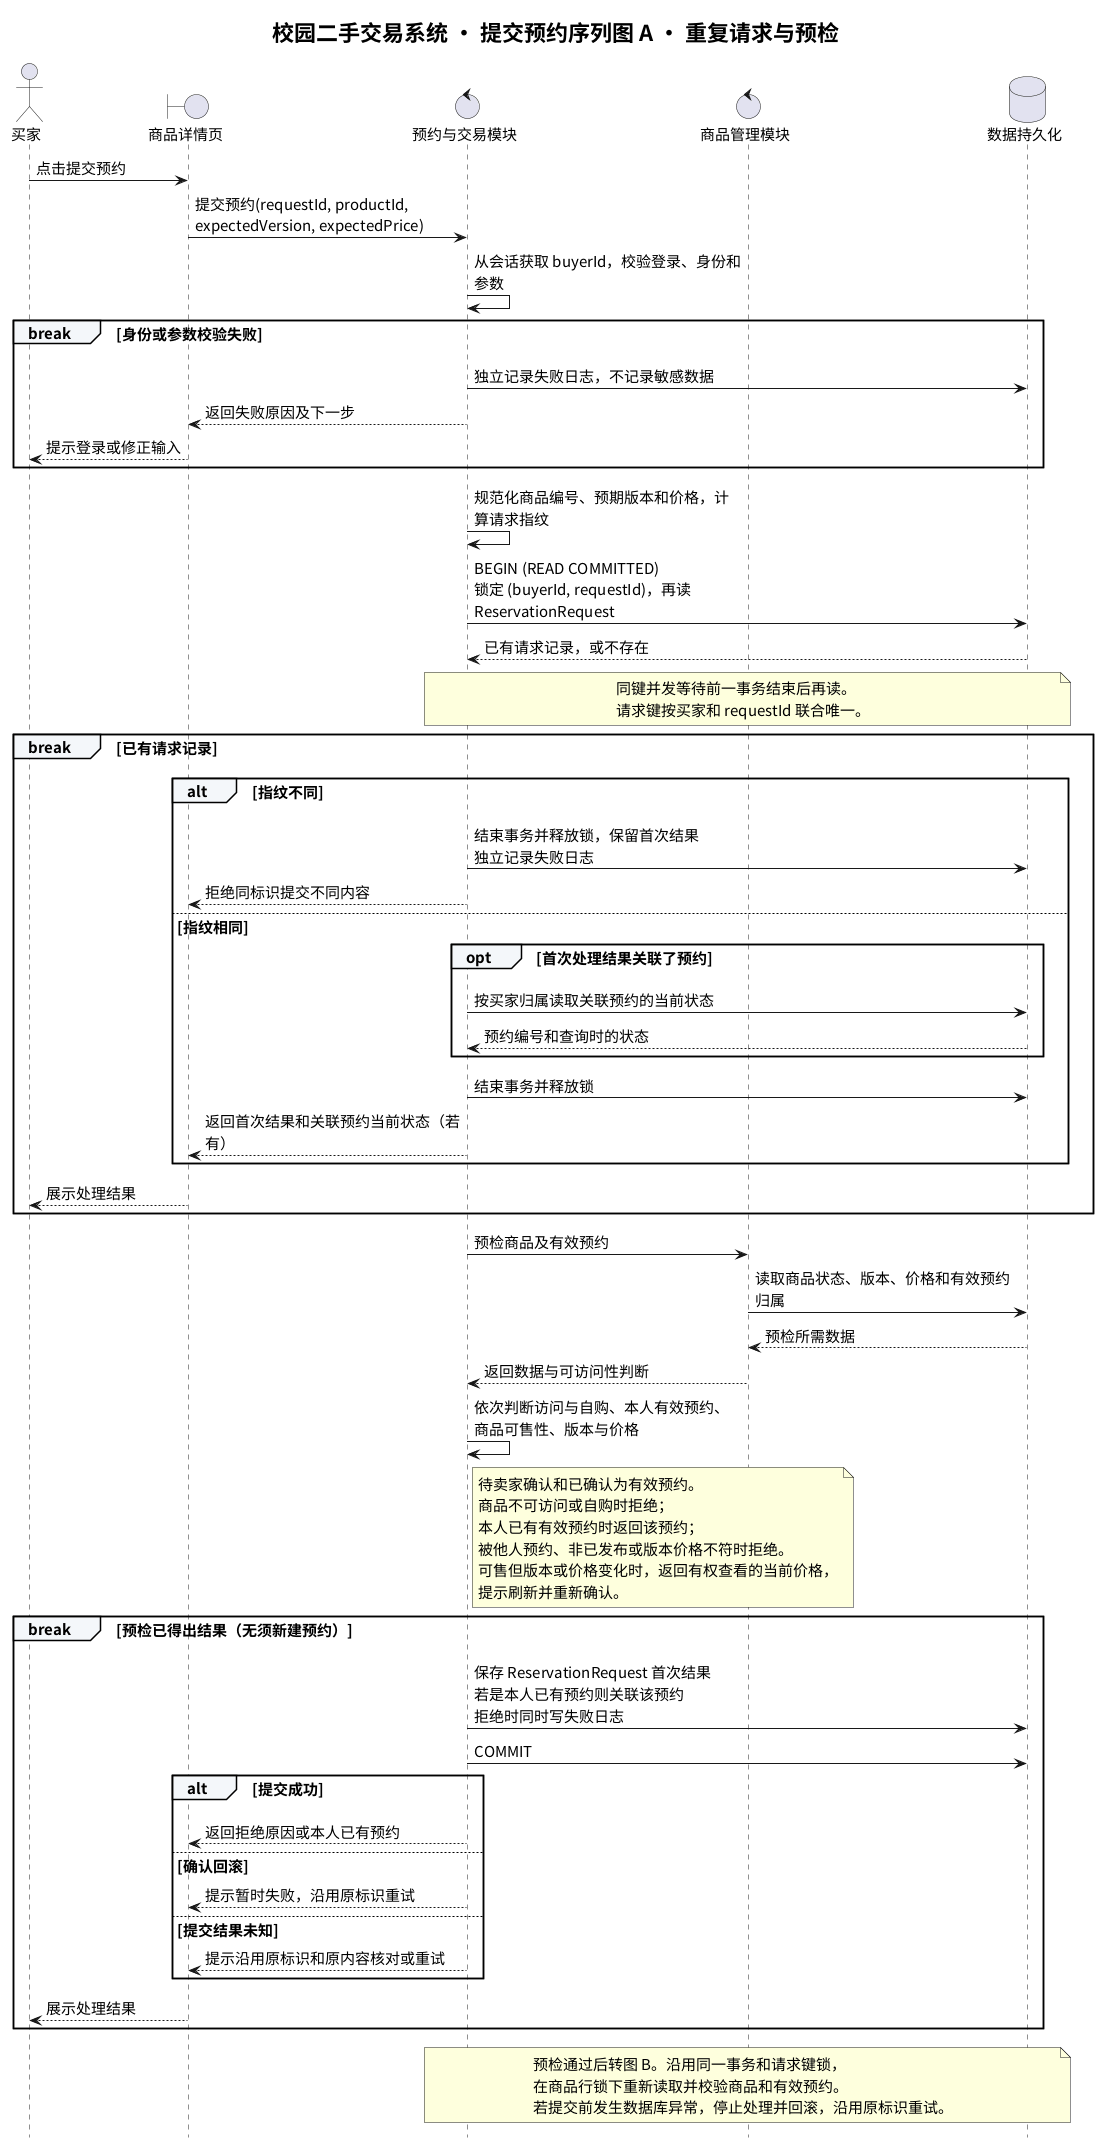
\includegraphics[width=\linewidth,height=0.70\textheight,keepaspectratio]{UML/提交预约序列图-A-重复请求与预检.png}
\caption{提交预约序列图 A：幂等与预检（交互性图）}
\end{figure}


\noindent\small 同标识不同内容拒绝；同内容重放首次结果并查询关联预约当前状态。新标识时先检查本人已有有效预约，再检查可售状态和版本价格。



\clearpage

\subsubsection{锁定复核、整体提交与通知}
图 B 延续图 A 的同一事务。初稿选用请求键互斥和商品行锁，锁定后重读当前数据；这一机制属于设计选择，要求其他相关写用例遵循相同锁协议。



\begin{figure}[H]
\centering
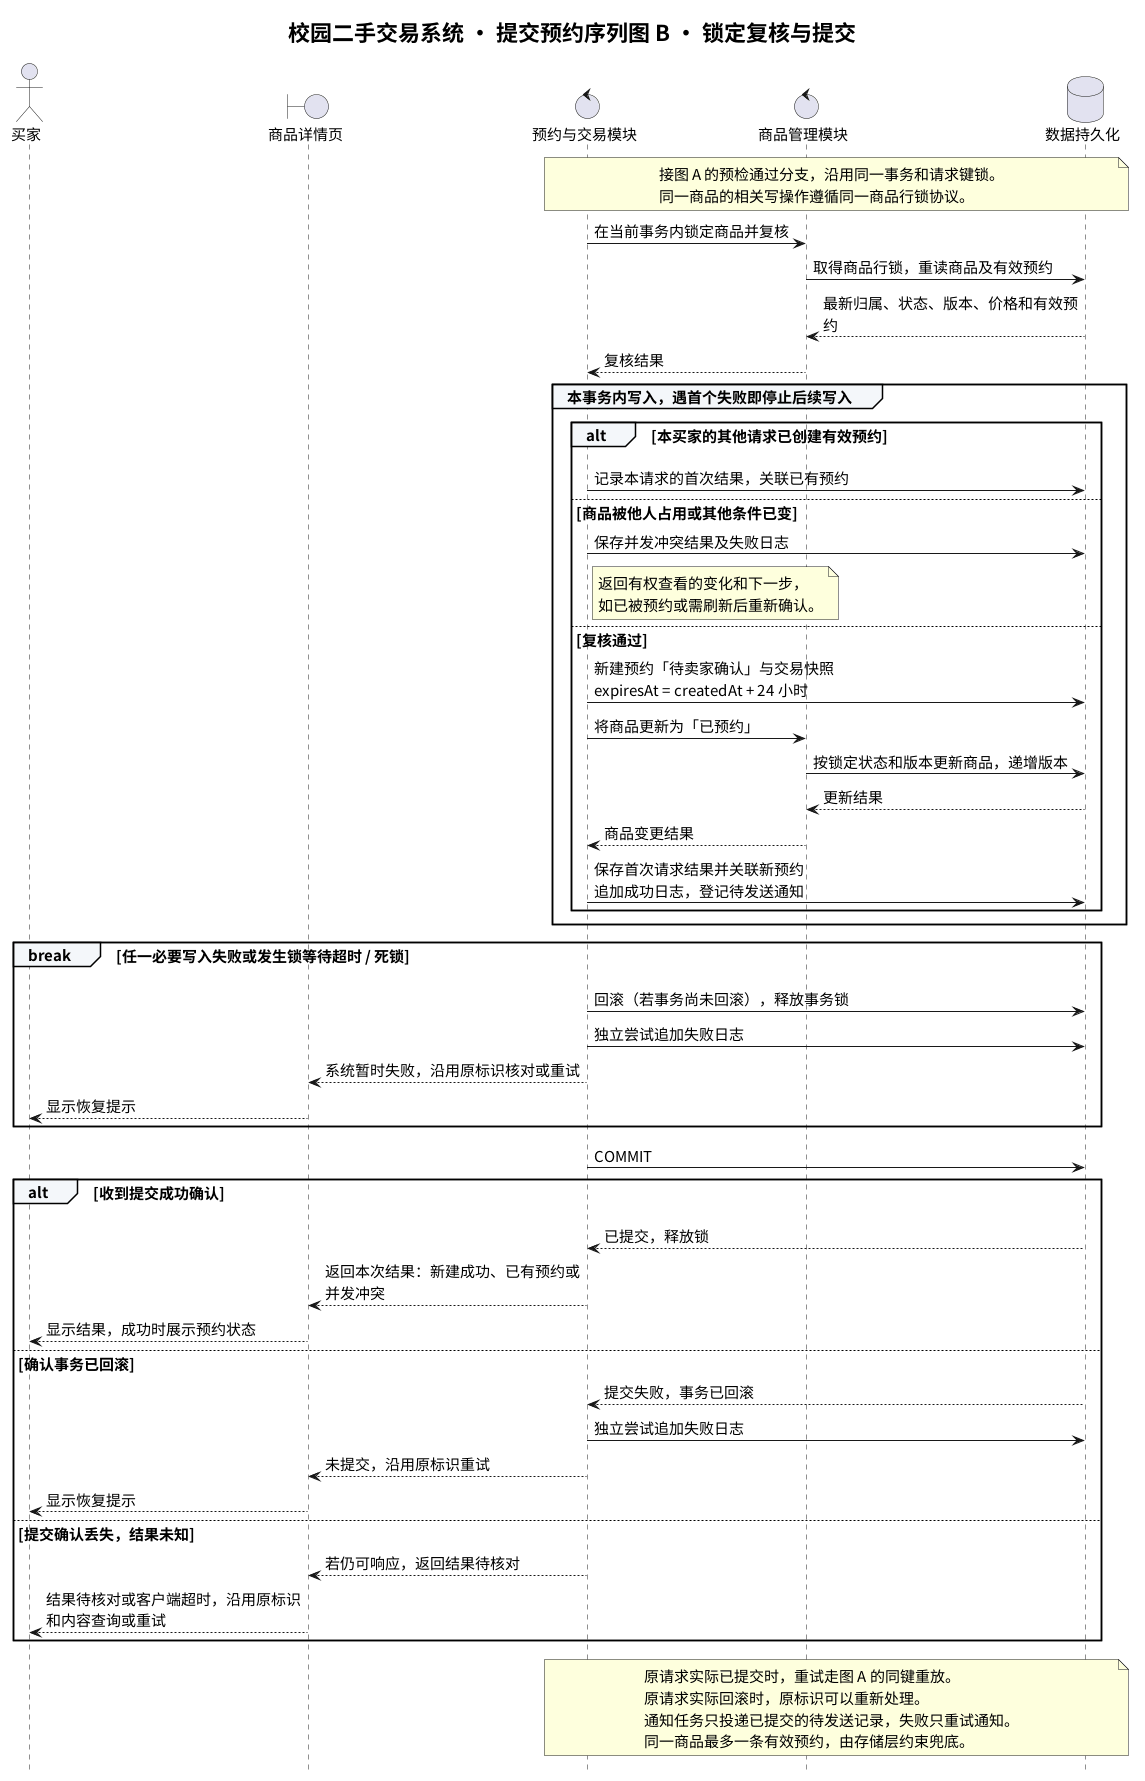
\includegraphics[width=\linewidth,height=0.68\textheight,keepaspectratio]{UML/提交预约序列图-B-锁定复核与提交.png}
\caption{提交预约序列图 B：复核与原子提交（交互性图）}
\end{figure}


\noindent\small 成功路径同事务保存预约快照、商品状态、请求结果、成功日志及待发送通知。提交确认丢失时返回结果待核对，沿用原标识重试；通知任务只处理已提交记录。



\clearpage

\subsubsection{失败分类与一致性设计的理由}
\begin{table}[H]\centering\small
\caption{提交预约的失败分类与恢复方式}
\begin{tabularx}{\linewidth}{@{}p{30mm}Y Y@{}}\toprule
分类 & 典型触发 & 恢复方式\\\midrule
普通校验失败 & 未登录、自购、商品不可售、预检时版本或价格已失效 & 给出原因；价格变化要求主动刷新和重新确认。\\
已有预约 & 新标识提交，但本人已存在有效预约 & 返回已有预约，不重复创建或重复登记成功事件。\\
并发竞争失败 & 预检通过后，锁定复核发现被占用或状态版本变化 & 返回有权查看的最新变化与下一步，不作为服务故障。\\
系统写入失败 & 数据库异常、必要写入失败、锁超时或死锁 & 整体回滚，独立尝试记录失败，原标识核对或重试。\\
提交结果未知 & 提交确认丢失或客户端网络超时 & 不断言成功或失败；沿用原标识及内容查结果或重试。\\\bottomrule
\end{tabularx}
\end{table}

只在前端禁用预约按钮无法保证并发唯一性，因为不同买家、旧页面或直接接口请求都可以绕过它。
因此，预检负责及时反馈，锁定复核负责重新判断，存储约束负责最终兜底。
请求键互斥还必须覆盖原记录不存在时的同键竞争，不能只对已经存在的记录加锁。

交易快照由服务端当前合法商品数据生成，提交价格仅用于与用户确认值比较，不能直接作为不受校验的成交金额。
状态或价格变更不允许系统静默接受新约定。

完整序列图用于连续查看全部分支和提交后通知路径；报告正文用 A/B 两段展示，避免整图压缩过小。


\clearpage

\section{UI 界面与功能描述}
\subsection{界面组织与设计约定}
原型以“校园集”为产品名，使用暖白底、深绿色操作按钮和低饱和状态标签。
桌面详情采用图片与信息双栏，卖家和管理员页面使用左侧导航与右侧工作区。
同一类操作保持按钮位置与语义一致，失效或完成后的操作按钮关闭。

现有截图覆盖账户、商品管理、审核与违规处置、查询展示、预约交易、通知、统计和日志八个模块。
下列截图直接使用现有导出材料；部分图片仅在报告副本中去除浏览器视口外的空白边，原始 PNG 不变。

\begin{table}[H]\centering\small
\caption{UI 功能与界面组织}
\begin{tabularx}{\linewidth}{@{}p{35mm}Y@{}}\toprule
功能 & 界面组织\\\midrule
买家预约与异常反馈 & 详情、确认、价格变化及不可预约状态\\
卖家发布与处理预约 & 发布商品和处理预约两个页面\\
管理员审核与违规处置 & 待审核列表、审核详情和违规下架页面\\
账户、列表、我的预约、通知、统计、日志及终止申请 & 通过补充界面导航切换各功能画面\\\bottomrule
\end{tabularx}
\end{table}

Figma Design 文件链接：\href{https://www.figma.com/design/UveEIuuGRnKhcVQPn48cLA/}{校园二手交易系统 · 实验二 UI}。
本稿以本地导出的24张 PNG 为图件来源，不把导出 PNG 等同于已验证线上所有图层可编辑。

\begin{keypoint}
不同画面可能来自不同演示时间和样本。例如，待审核结果的相机价格为1600元，预约与管理演示常为1680元，补充列表为1780元。
这些图片不是同一数据库记录的连续运行截图，不能据此声称价格快照或事务已在真实后端验证。
\end{keypoint}


\clearpage

\subsection{账户与权限：登录、注册}
登录提供用户名和密码入口，注册收集用户名、昵称、密码及交易联系方式。
普通账号可同时买卖；管理员账号不通过普通注册产生。联系方式只按交易关联和状态授权访问。




\begin{figure}[H]
\centering
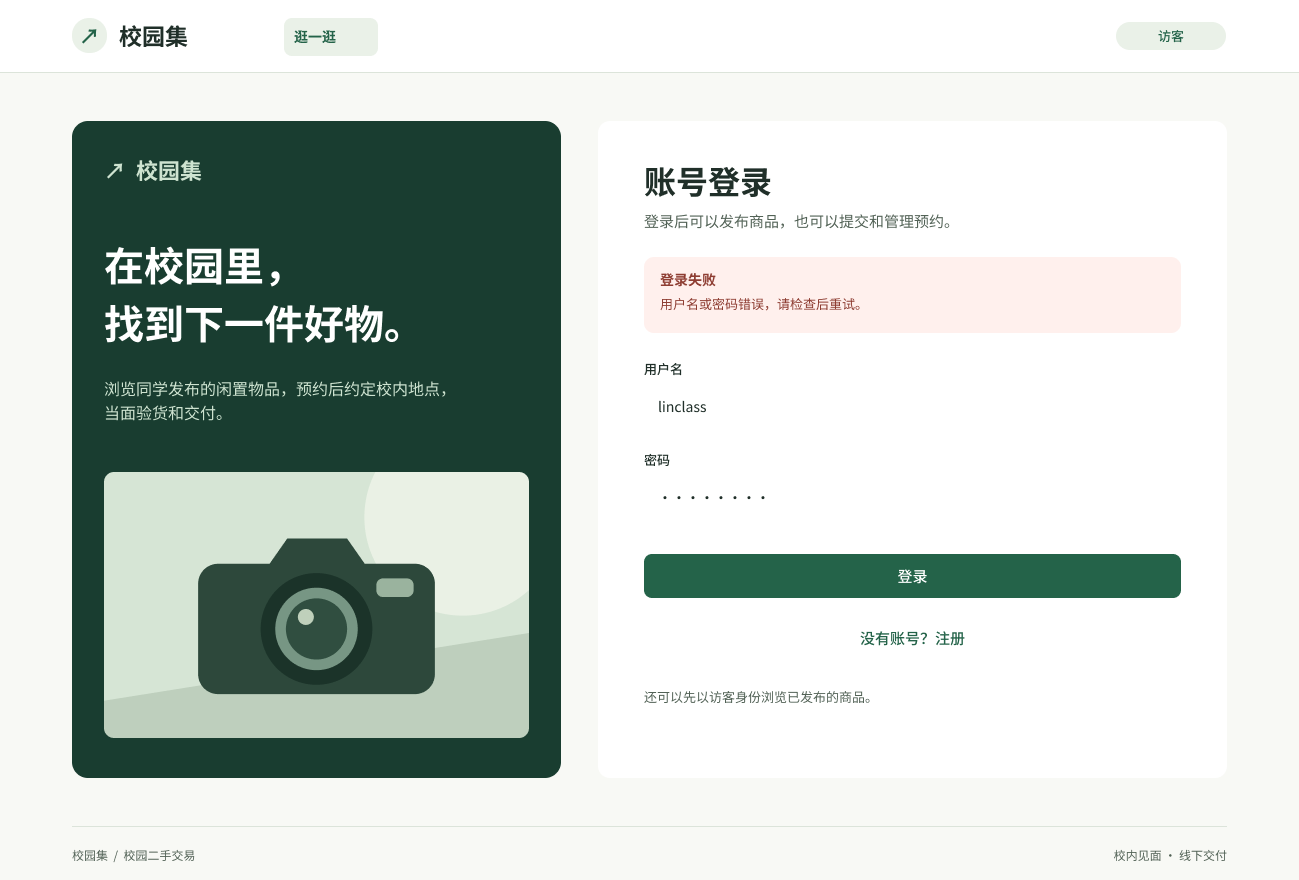
\includegraphics[width=\linewidth,height=0.34\textheight,keepaspectratio]{Report/assets/ui-01.png}
\caption{登录界面：访客登录与注册入口}
\end{figure}



\begin{figure}[H]
\centering
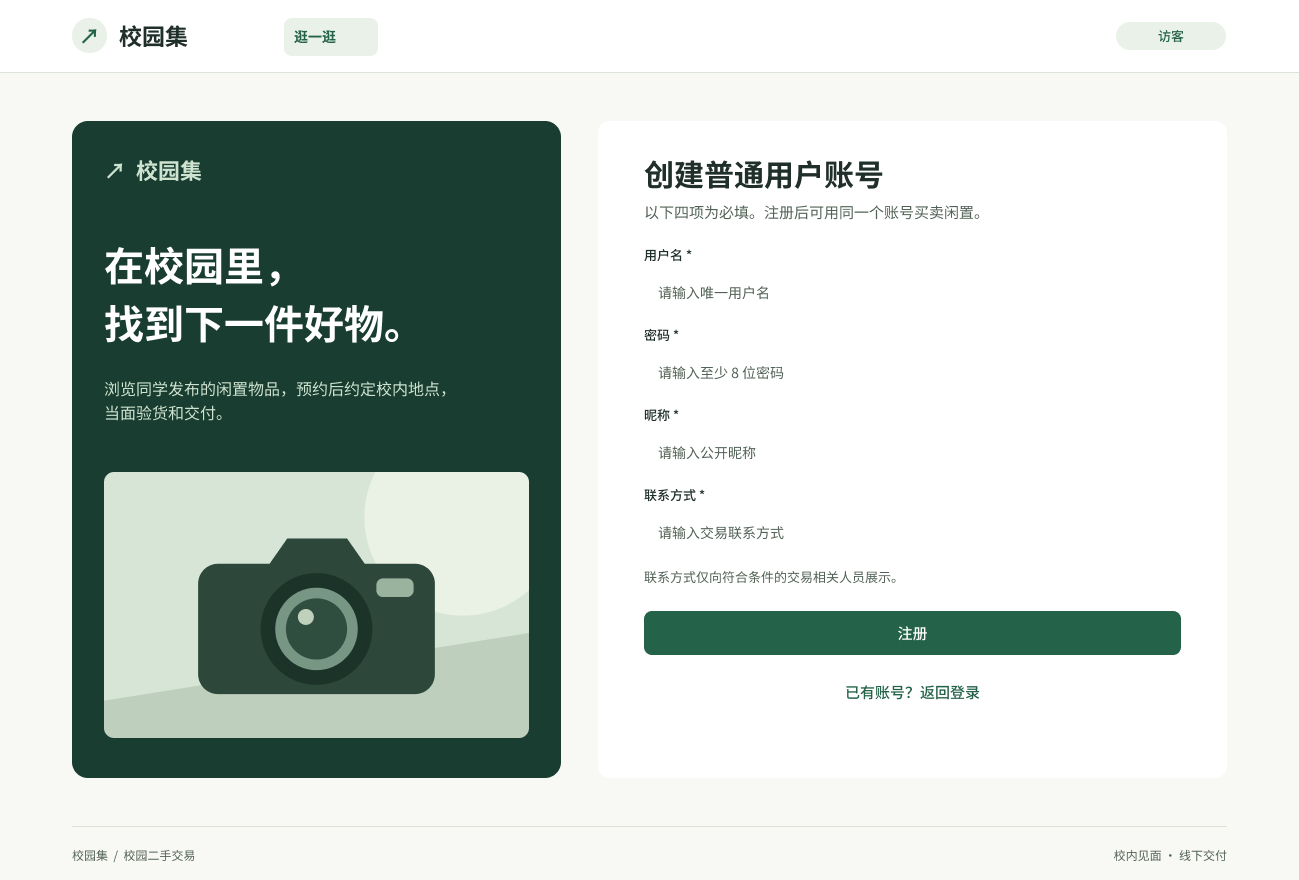
\includegraphics[width=\linewidth,height=0.34\textheight,keepaspectratio]{Report/assets/ui-02.png}
\caption{注册界面：普通用户账户信息}
\end{figure}


\clearpage

\subsection{查询与展示：列表筛选及商品详情}
列表组织关键词、分类、价格区间、状态、排序和分页入口；公开查询仅返回已发布商品。
详情展示描述、图片、价格和交付地点，不公开联系方式。各筛选条件须同时成立，分页排序应稳定。




\begin{figure}[H]
\centering
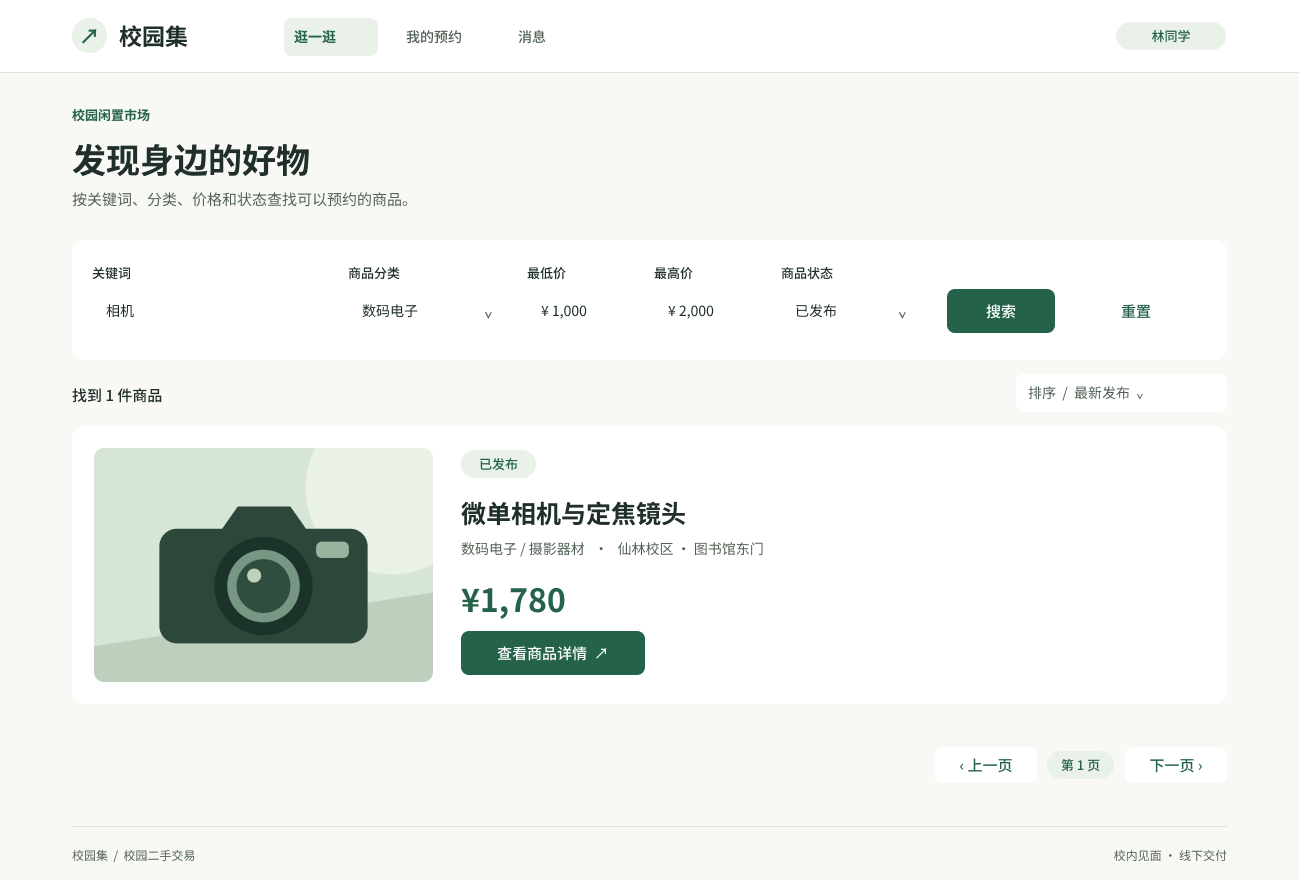
\includegraphics[width=\linewidth,height=0.34\textheight,keepaspectratio]{Report/assets/ui-03.png}
\caption{商品列表与组合搜索}
\end{figure}



\begin{figure}[H]
\centering
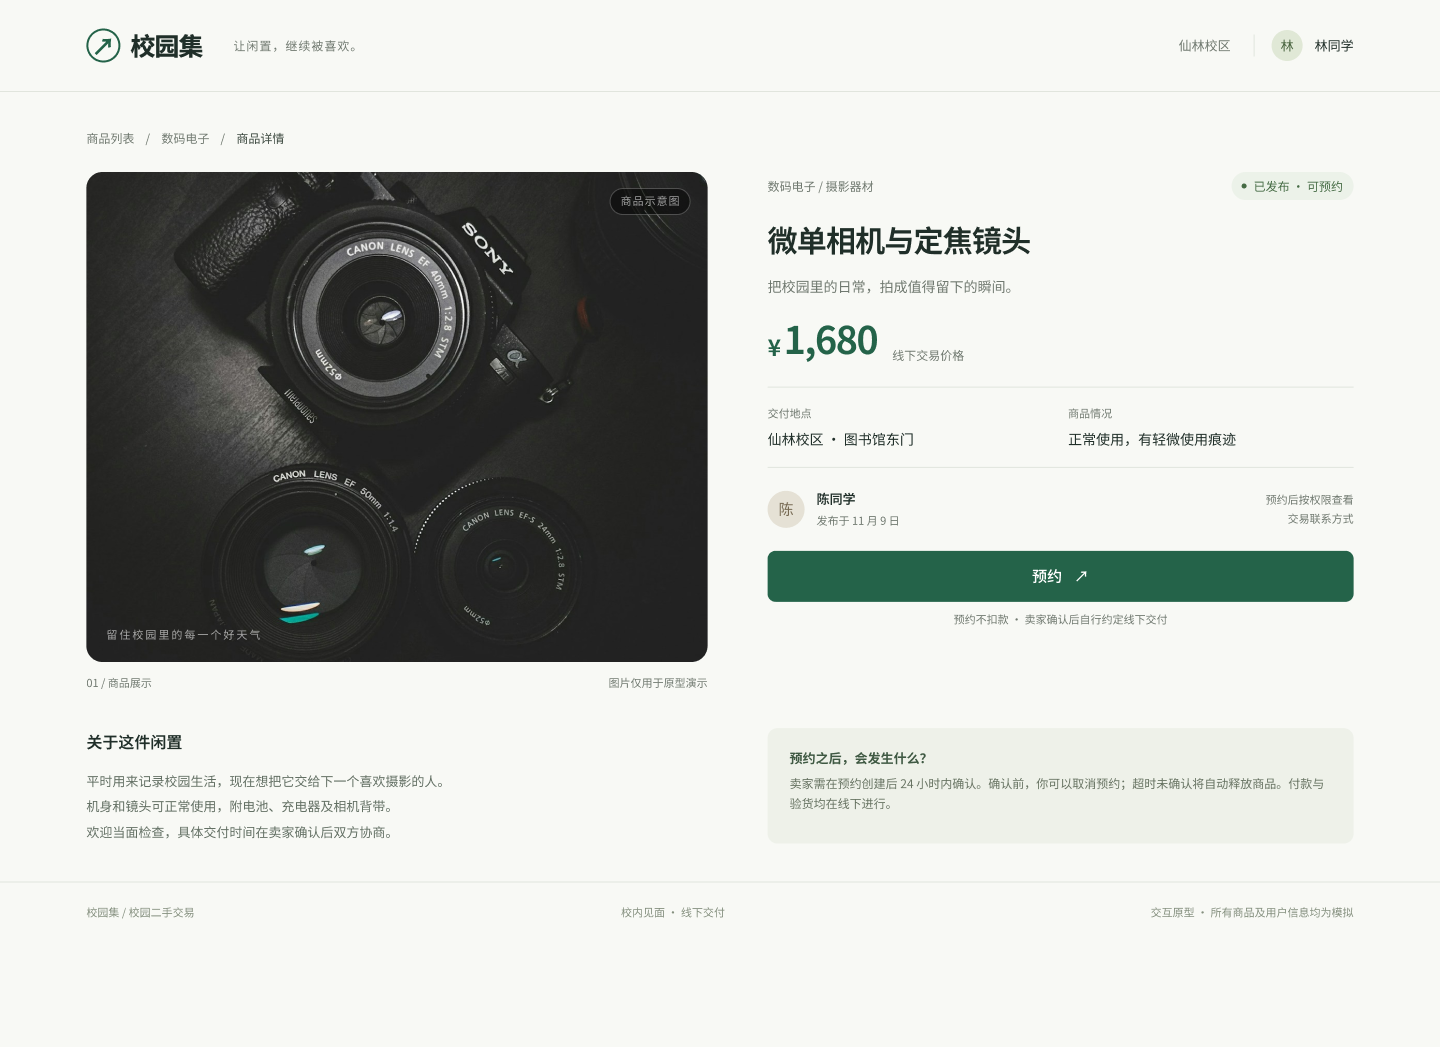
\includegraphics[width=\linewidth,height=0.34\textheight,keepaspectratio]{Report/assets/ui-04.png}
\caption{商品详情与预约入口}
\end{figure}


\clearpage

\subsection{预约创建：确认与等待卖家确认}
买家点击预约后先核对本次价格，确认前可取消弹窗。
提交成功后展示待卖家确认，商品进入已预约；该成功画面不是再次打开未提交的确认弹窗。
预约不扣款，卖家确认后双方自行约定线下交付。




\begin{figure}[H]
\centering
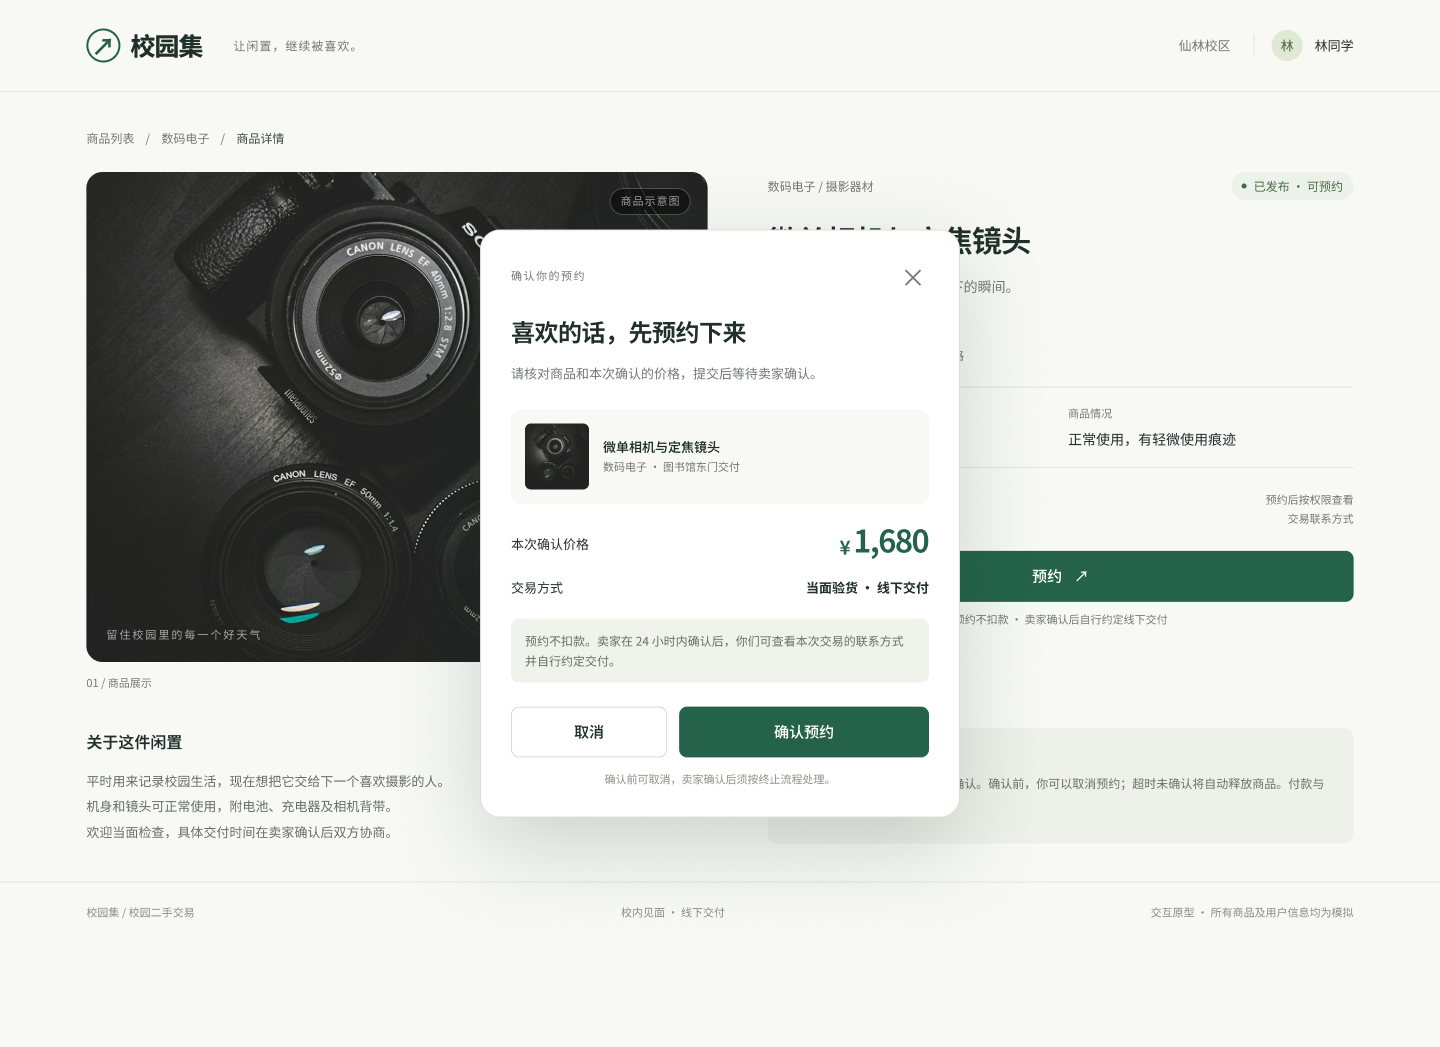
\includegraphics[width=\linewidth,height=0.34\textheight,keepaspectratio]{Report/assets/ui-05.png}
\caption{预约确认弹窗：本次确认价格与取消、确认按钮}
\end{figure}



\begin{figure}[H]
\centering
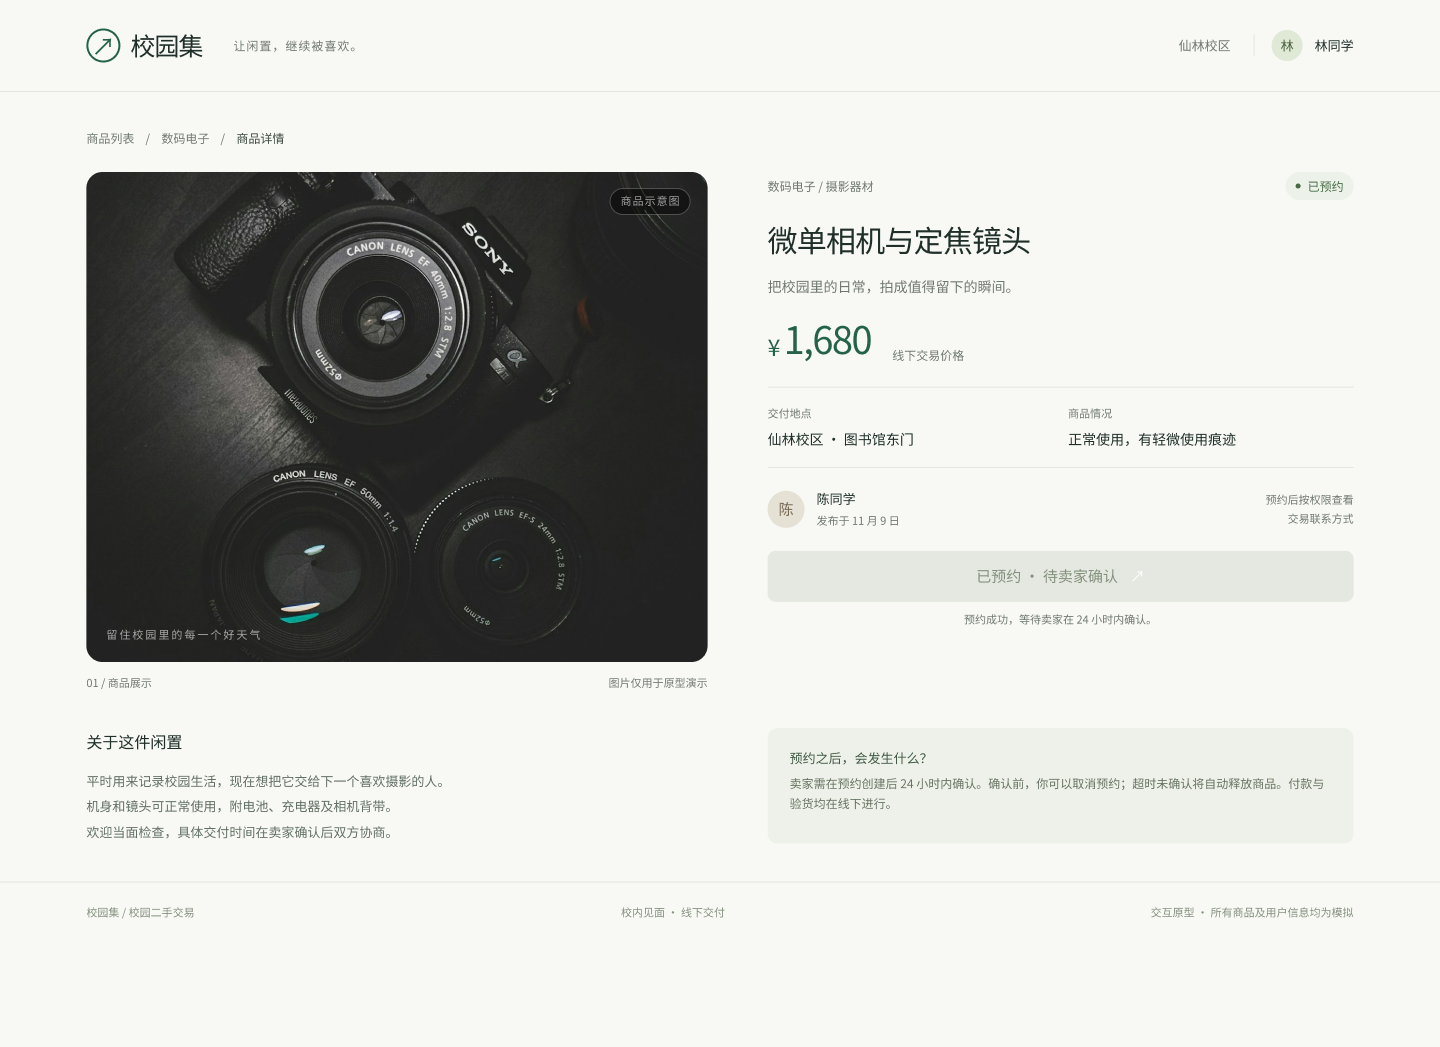
\includegraphics[width=\linewidth,height=0.34\textheight,keepaspectratio]{Report/assets/ui-06.png}
\caption{提交成功后的等待卖家确认画面}
\end{figure}


\clearpage

\subsection{预约异常：价格变化与他人占用}
旧价格失效时同时显示原价、现价和“本次未创建预约”的反馈，必须由买家主动重新确认。
他人已成功预约时给出明确的不可预约原因和返回列表入口，不将正常业务竞争显示为系统故障。




\begin{figure}[H]
\centering
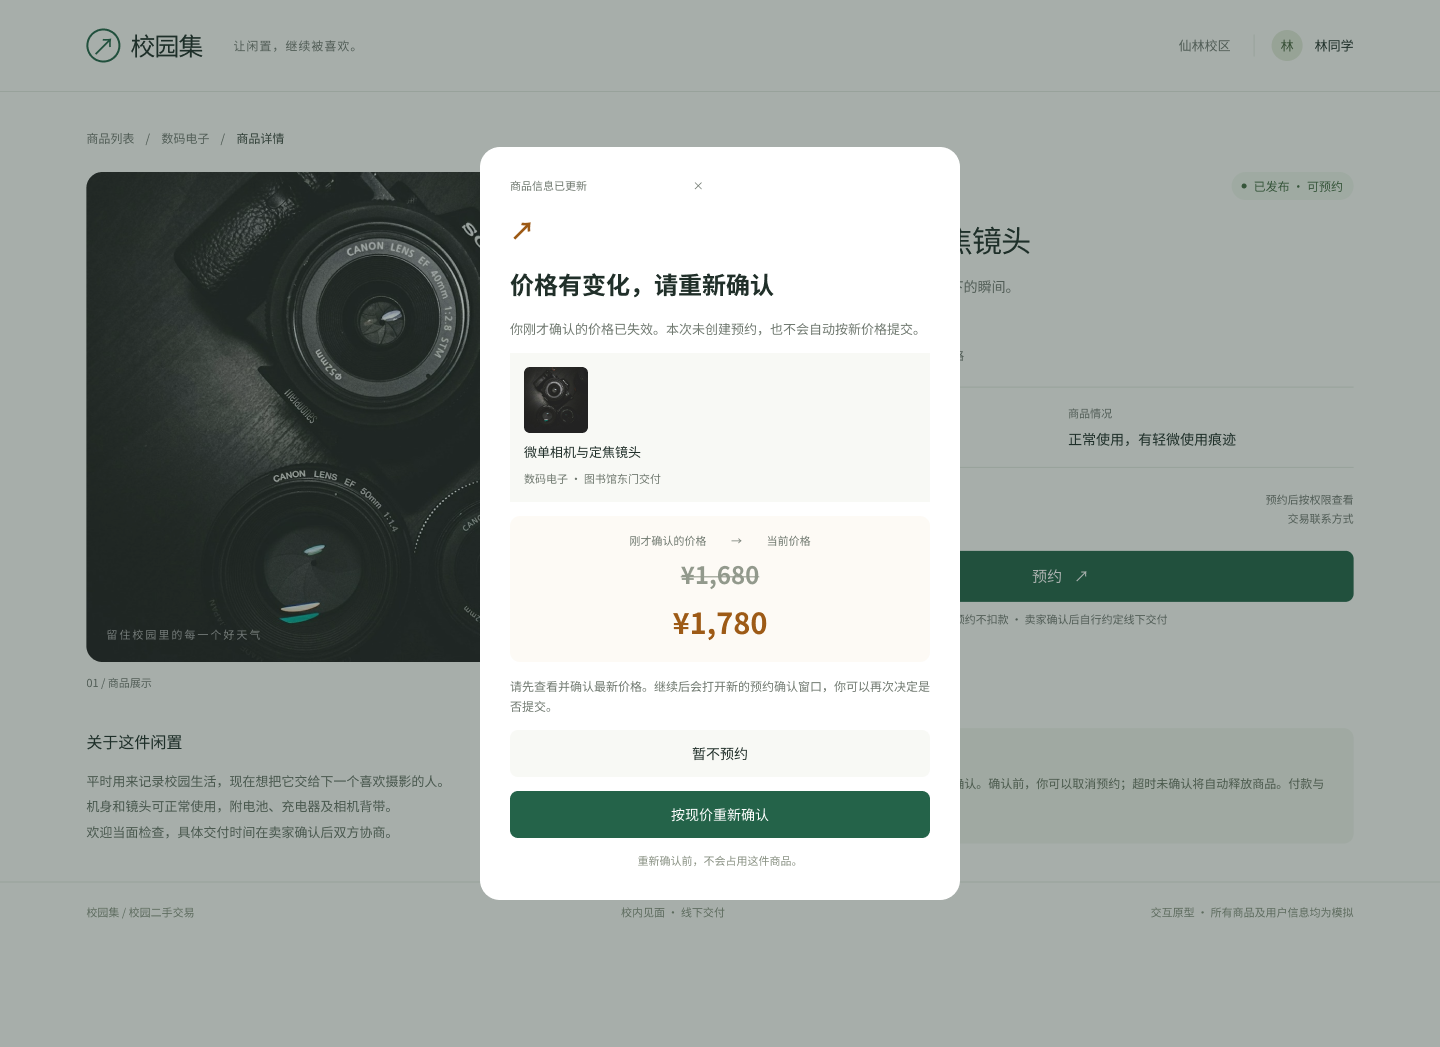
\includegraphics[width=\linewidth,height=0.34\textheight,keepaspectratio]{Report/assets/ui-07.png}
\caption{价格变化：展示原价与现价，重新确认后才可提交}
\end{figure}



\begin{figure}[H]
\centering
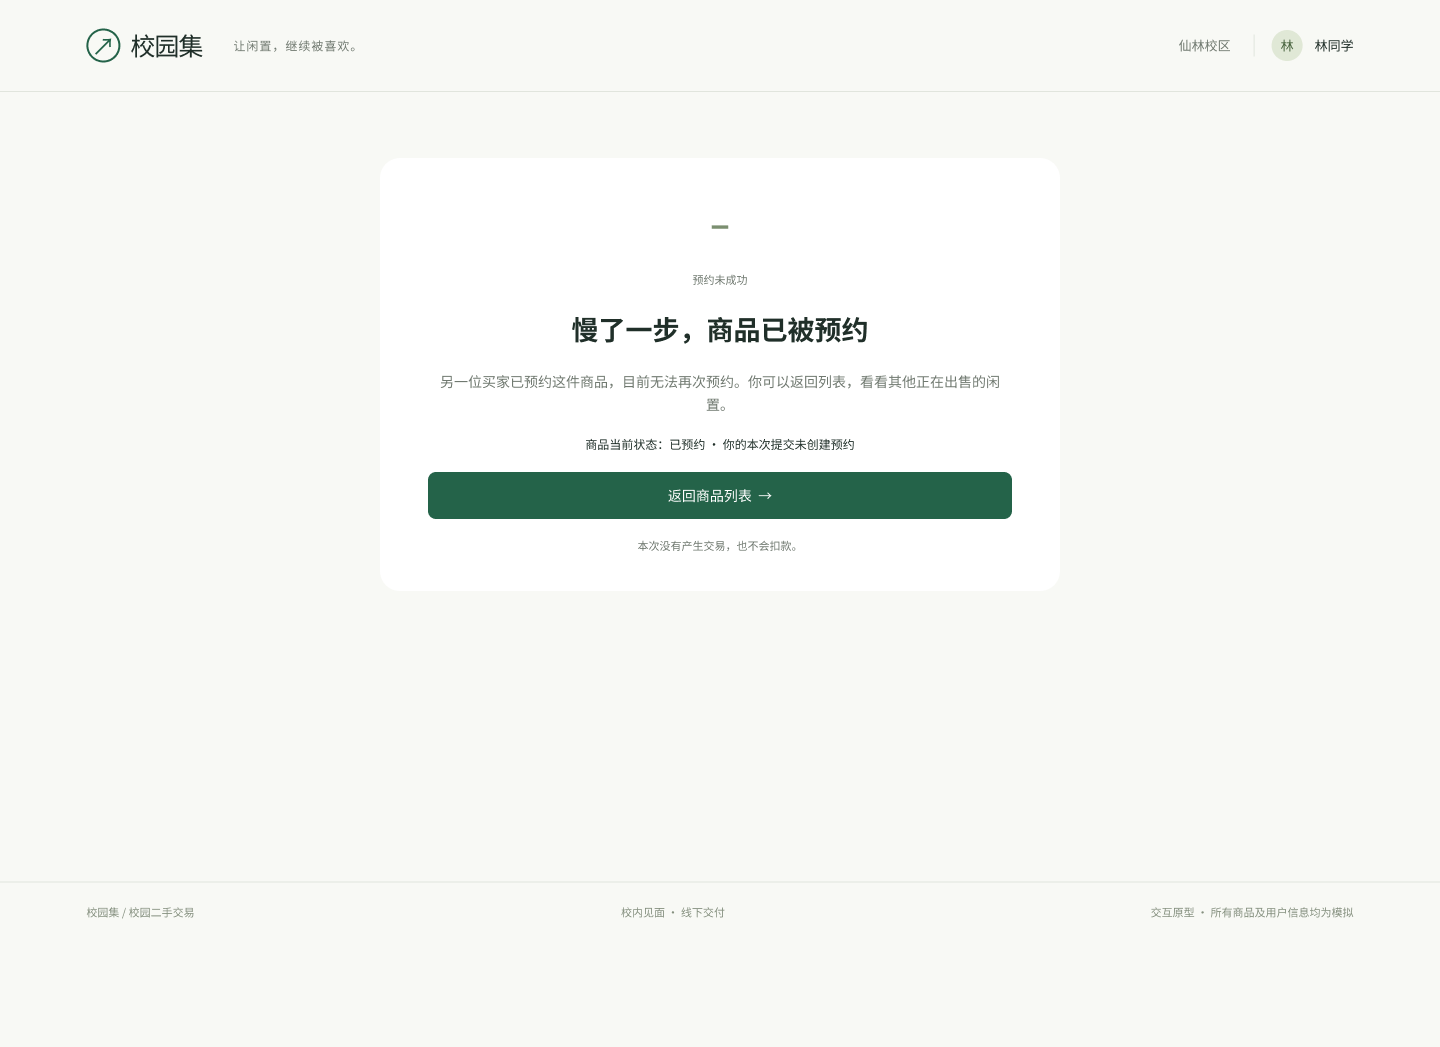
\includegraphics[width=\linewidth,height=0.34\textheight,keepaspectratio]{Report/assets/ui-08.png}
\caption{商品已被他人预约：明确结果与返回列表入口}
\end{figure}


\clearpage

\subsection{商品管理：发布表单与草稿}
卖家填写标题、描述、分类、价格、交付地点和图片。
草稿可缺字段，已填写字段仍要合法；草稿保存在本机浏览器用于原型演示，不能视为真实服务器持久化。
送审要求标题不超过100字、描述不超过2000字、图片1至5张、价格大于0且不超过10万元并最多两位小数。




\begin{figure}[H]
\centering
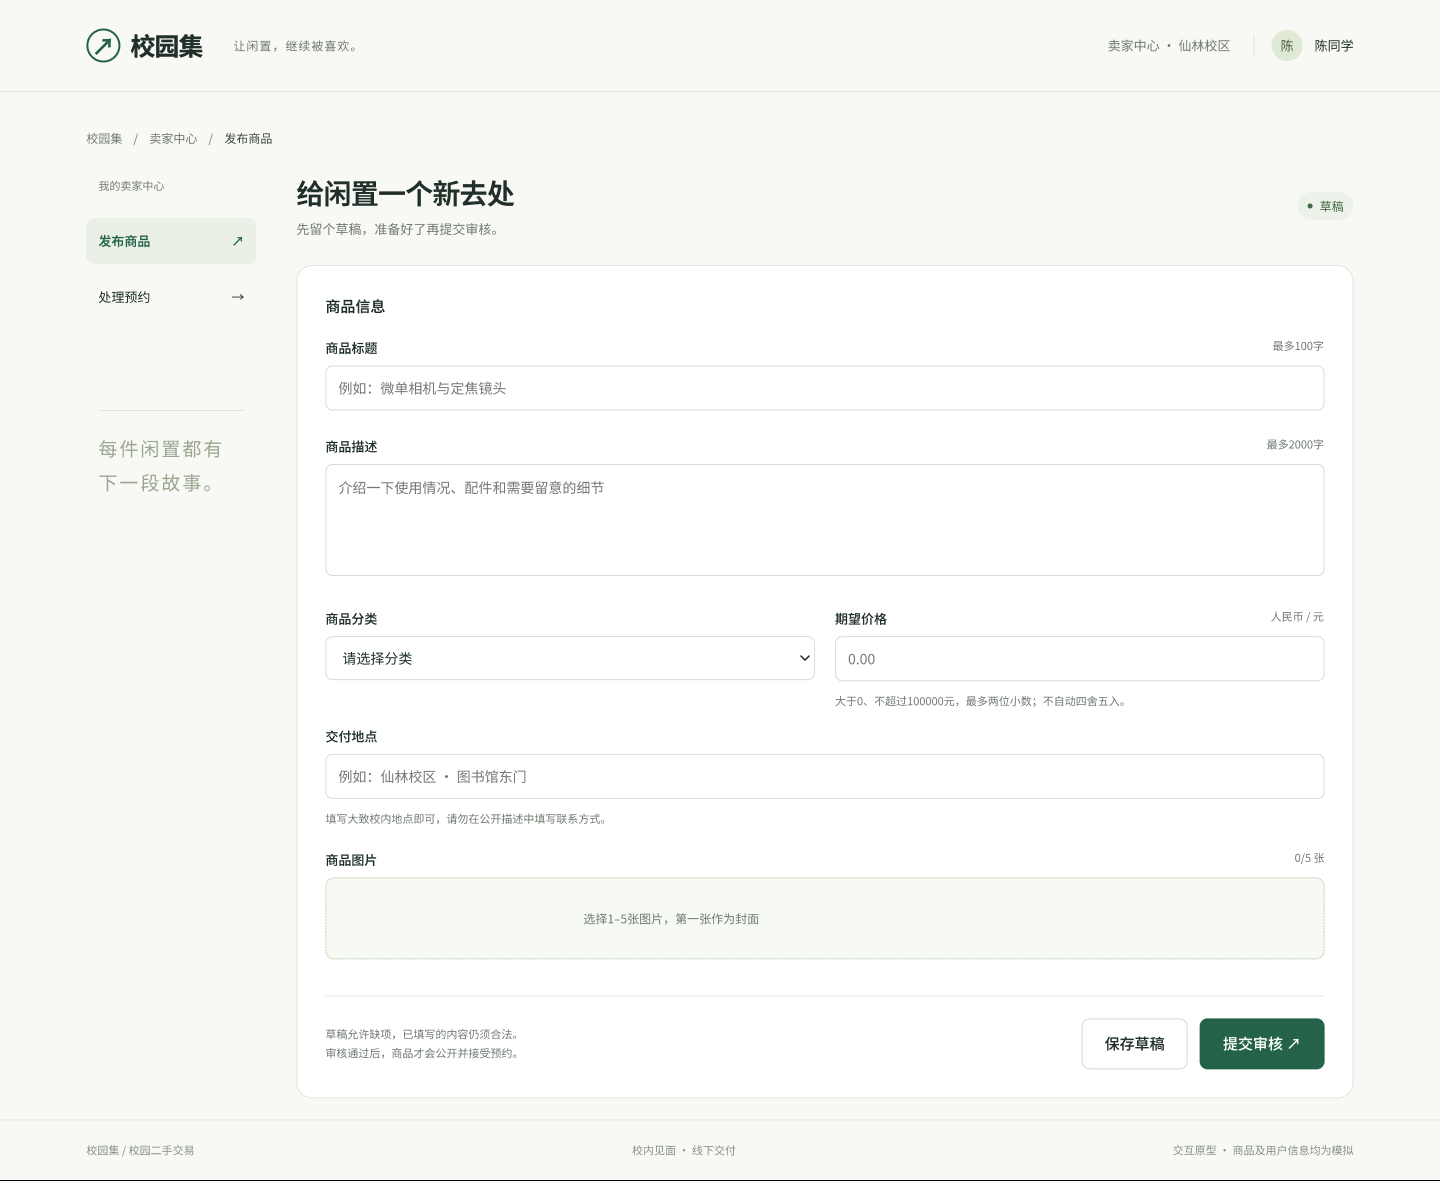
\includegraphics[width=\linewidth,height=0.66\textheight,keepaspectratio]{Report/assets/ui-09.png}
\caption{发布商品表单与保存草稿、提交审核入口}
\end{figure}


\clearpage

\subsubsection{送审校验与缺项草稿反馈}
该截图展示价格、图片缺失时的字段级错误，保留其他输入便于修正。
同一份缺项信息可以保存为草稿，但不能送审。
现有导出同时含“草稿已保存”和再次送审的错误提示，说明两个动作不同；最终展示时可将这两个状态分别捕获，以减少歧义。



\begin{figure}[H]
\centering
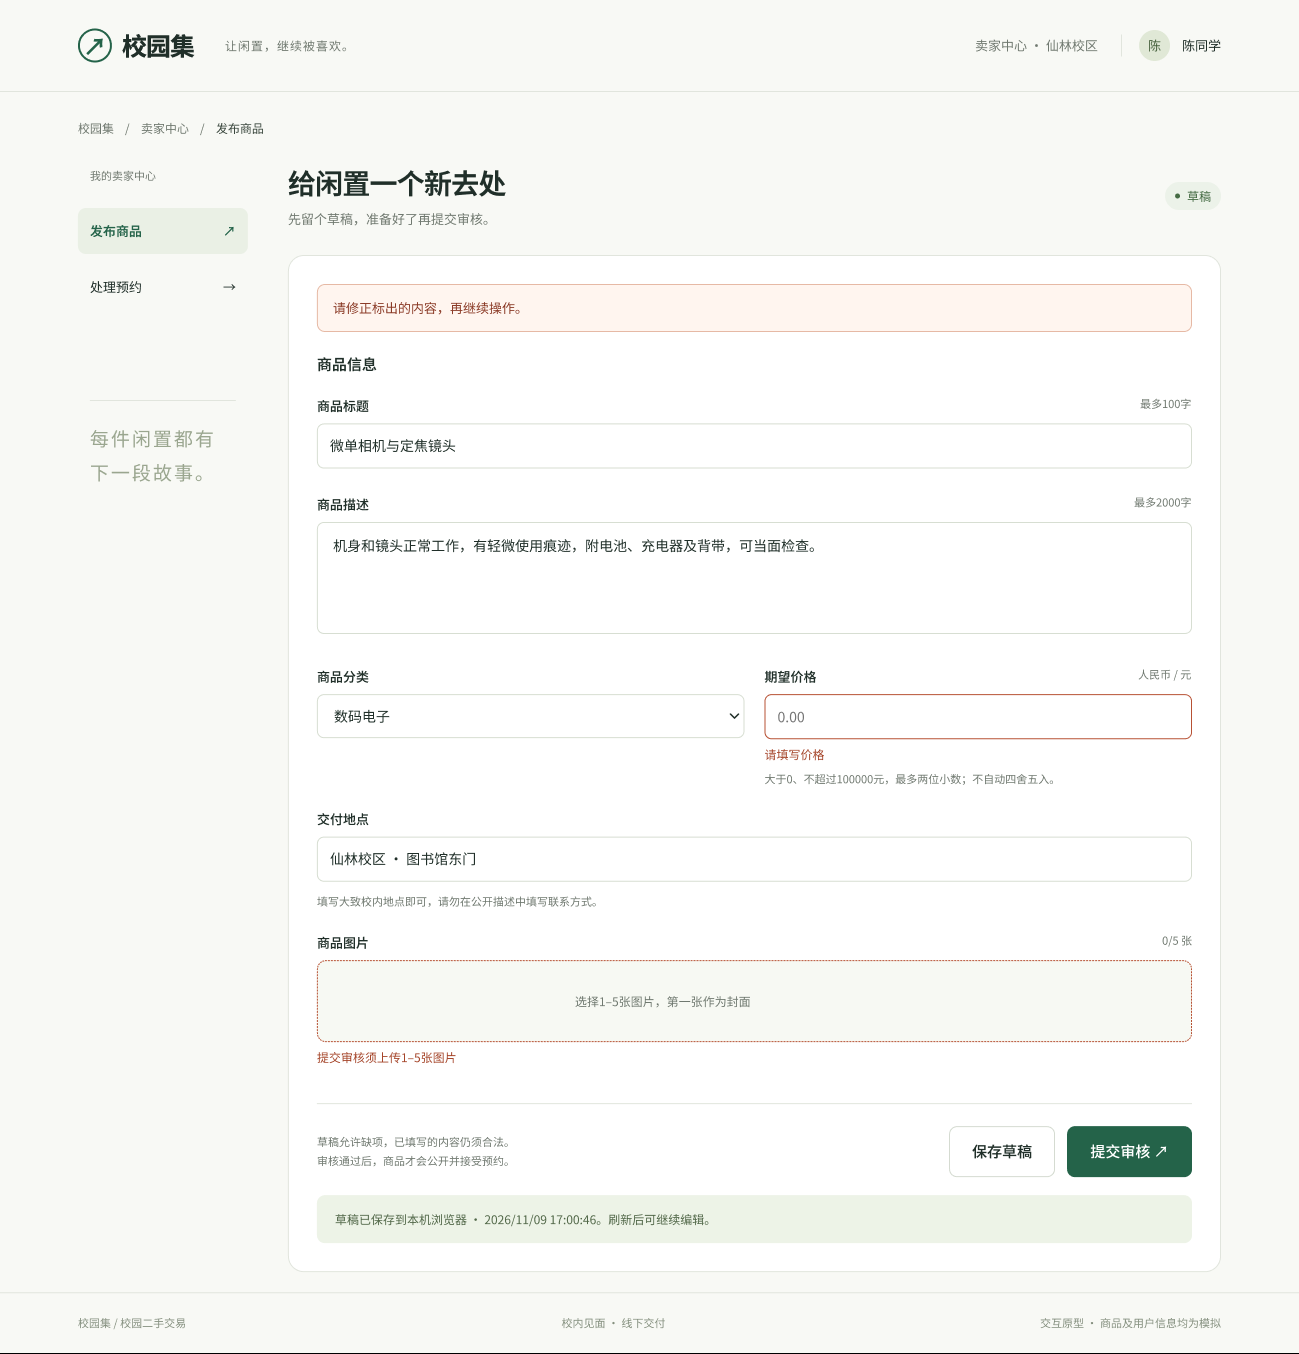
\includegraphics[width=\linewidth,height=0.69\textheight,keepaspectratio]{Report/assets/ui-10.png}
\caption{发布商品：缺价格与图片的校验反馈、草稿保存提示}
\end{figure}


\clearpage

\subsubsection{提交审核后的结果}
校验通过后商品变待审核，不再提供公开预约；界面给出“等待审核”的阶段提示。
待审核商品如需修改，应先撤回为草稿，不能直接改字段或跳过管理员审核发布。




\begin{figure}[H]
\centering
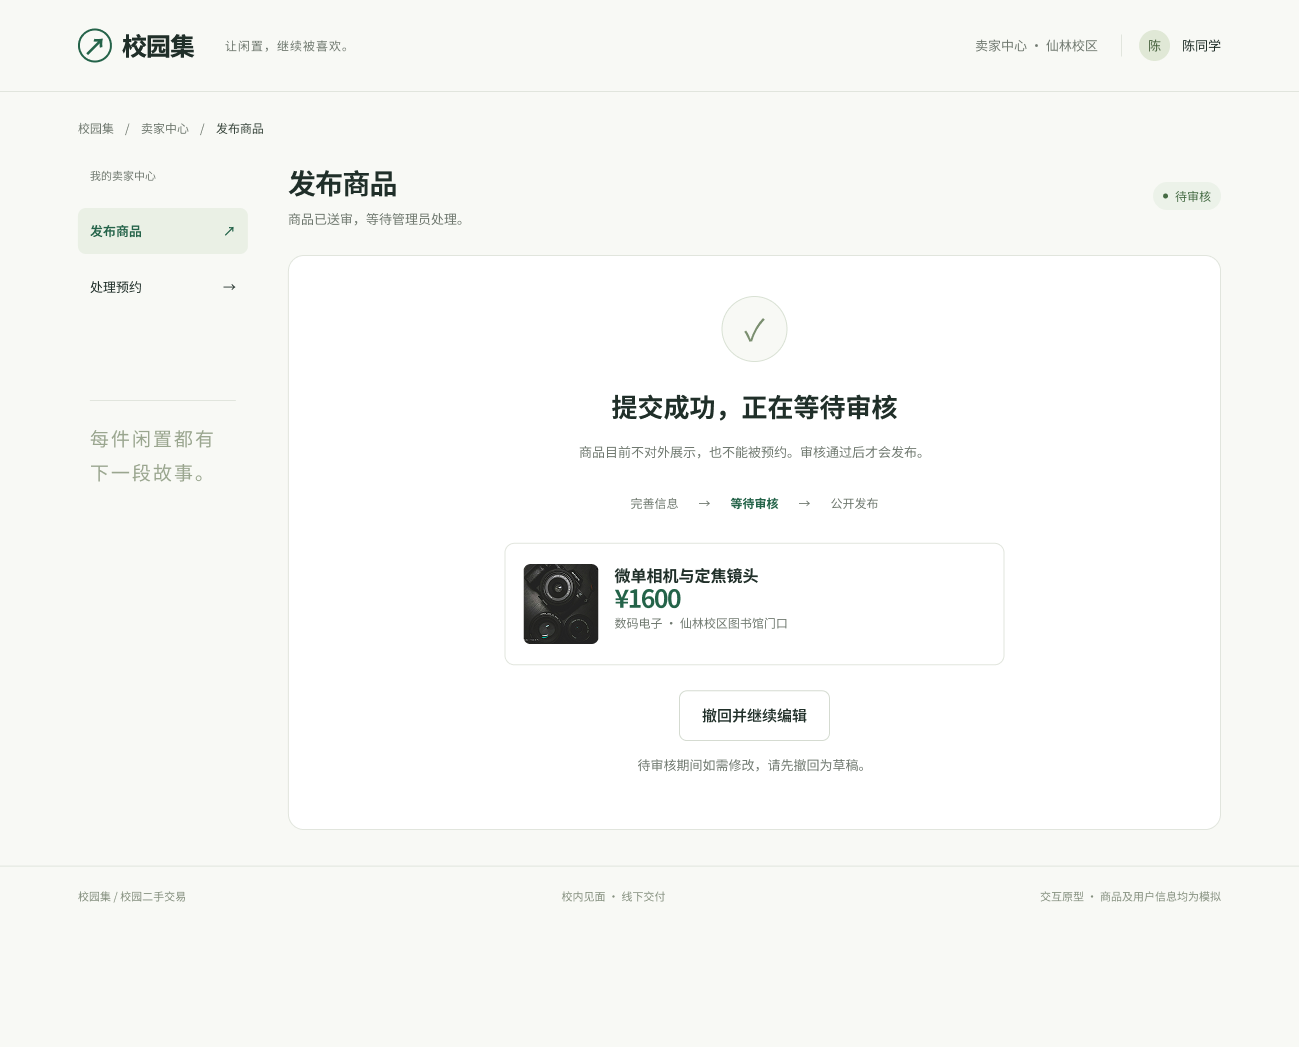
\includegraphics[width=\linewidth,height=0.65\textheight,keepaspectratio]{Report/assets/ui-11.png}
\caption{商品成功送审：待审核结果及撤回入口}
\end{figure}


\clearpage

\subsection{卖家处理预约：截止时间与操作入口}
预约卡片显示买家、价格快照、创建时间和北京时间截止时间。
确认或拒绝只允许待卖家确认状态且未到期；界面倒计时与提交时二次判断共同展示边界。
达到截止时刻后关闭两项操作，真实实现还须服务端按当前状态和时间复核。




\begin{figure}[H]
\centering
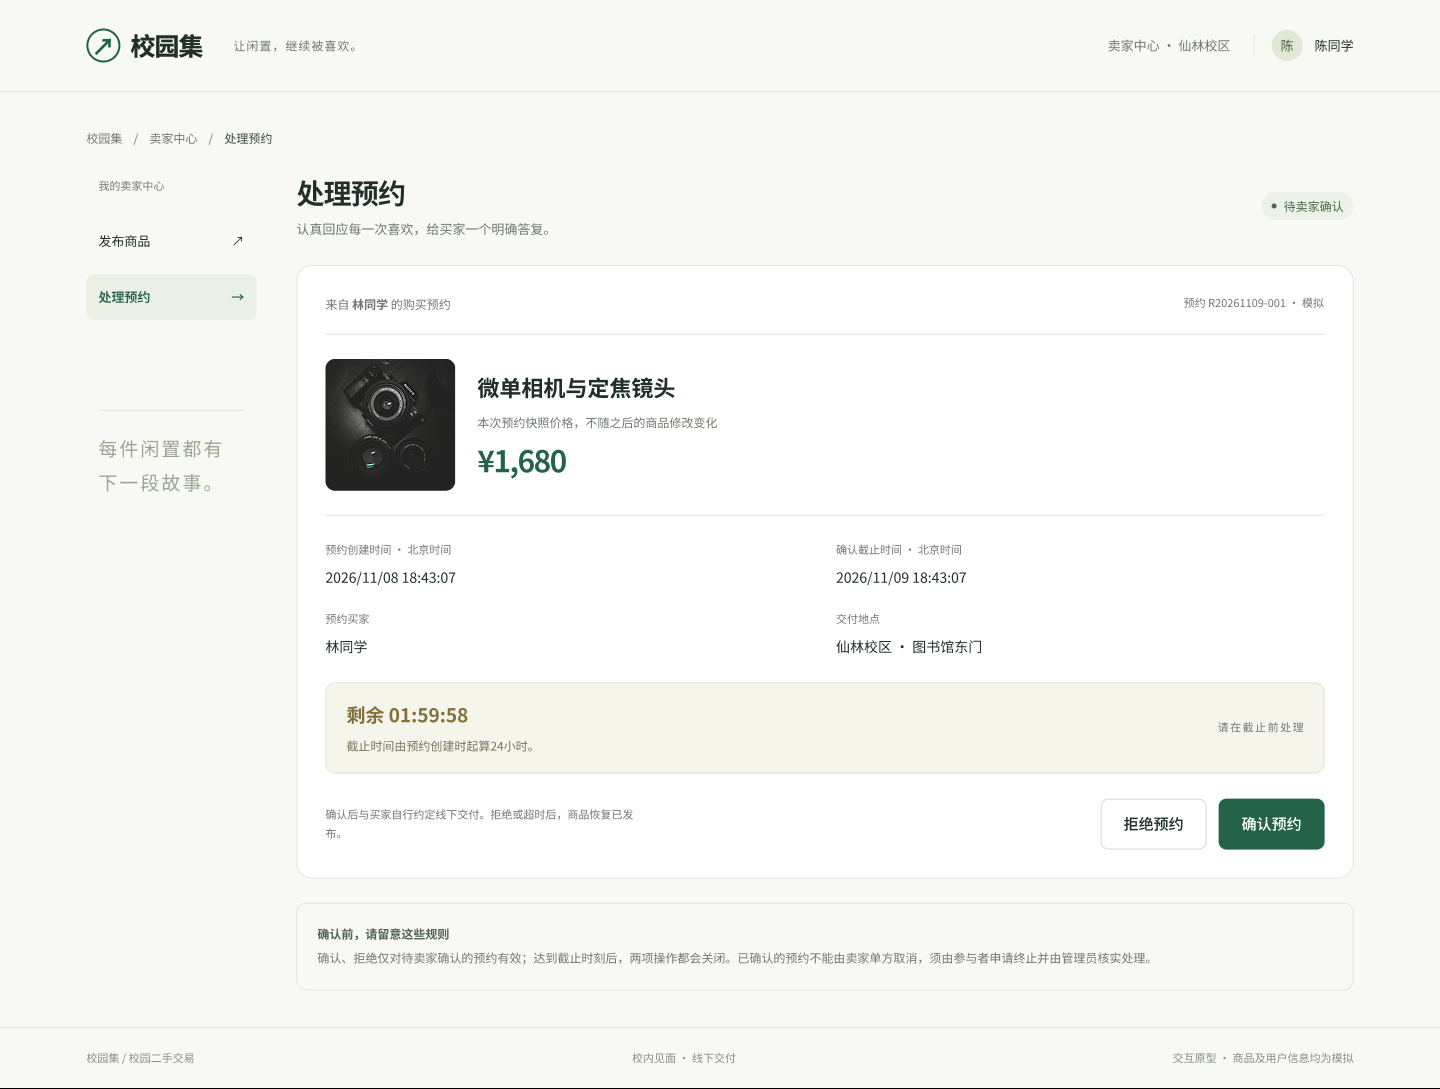
\includegraphics[width=\linewidth,height=0.66\textheight,keepaspectratio]{Report/assets/ui-12.png}
\caption{待卖家确认的预约与确认、拒绝入口}
\end{figure}


\clearpage

\subsubsection{拒绝结果与状态关闭}
拒绝必须填写非空原因，处理成功后预约已拒绝、商品恢复已发布，并通知买家。
已处理的预约关闭确认与拒绝入口，避免重复操作。
现有截图中的拒绝文案仅是演示输入；用于正式展示时宜采用具体客观的业务原因。



\begin{figure}[H]
\centering
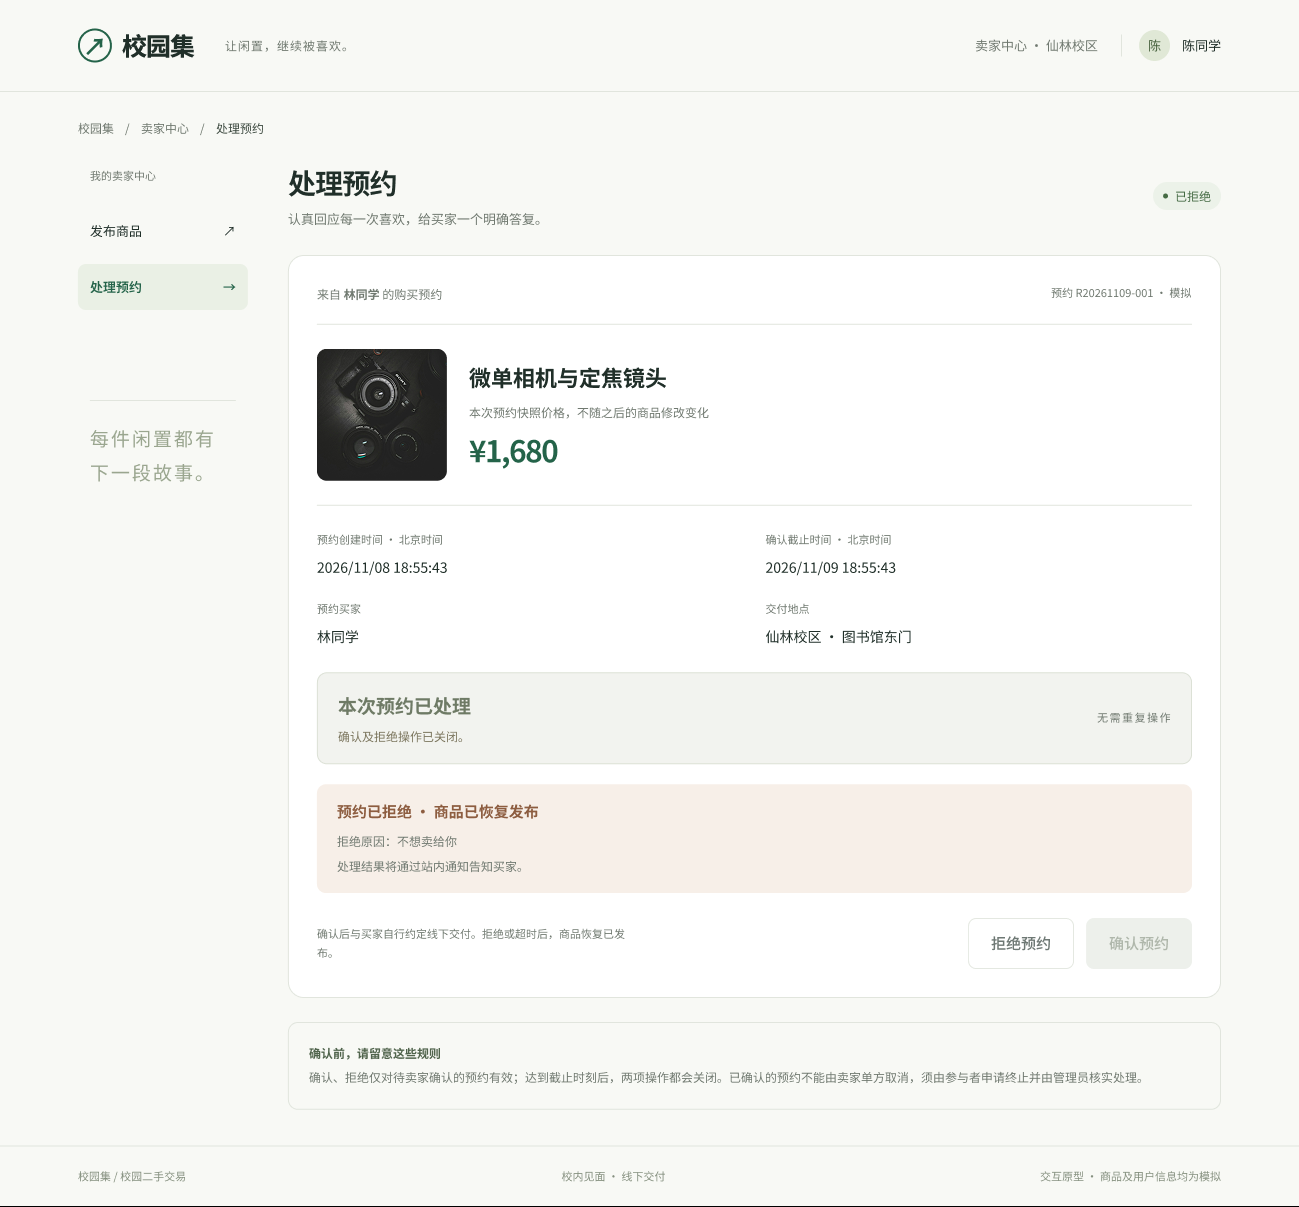
\includegraphics[width=\linewidth,height=0.68\textheight,keepaspectratio]{Report/assets/ui-13.png}
\caption{卖家拒绝预约后的结果与禁用操作}
\end{figure}


\clearpage

\subsection{审核管理：待审核列表}
管理员从待审核队列进入商品详情，列表展示商品、卖家、送审时间和状态。
商品一旦撤回或被处理，就不能继续从旧页面重复审核；状态检查须由服务端执行。




\begin{figure}[H]
\centering
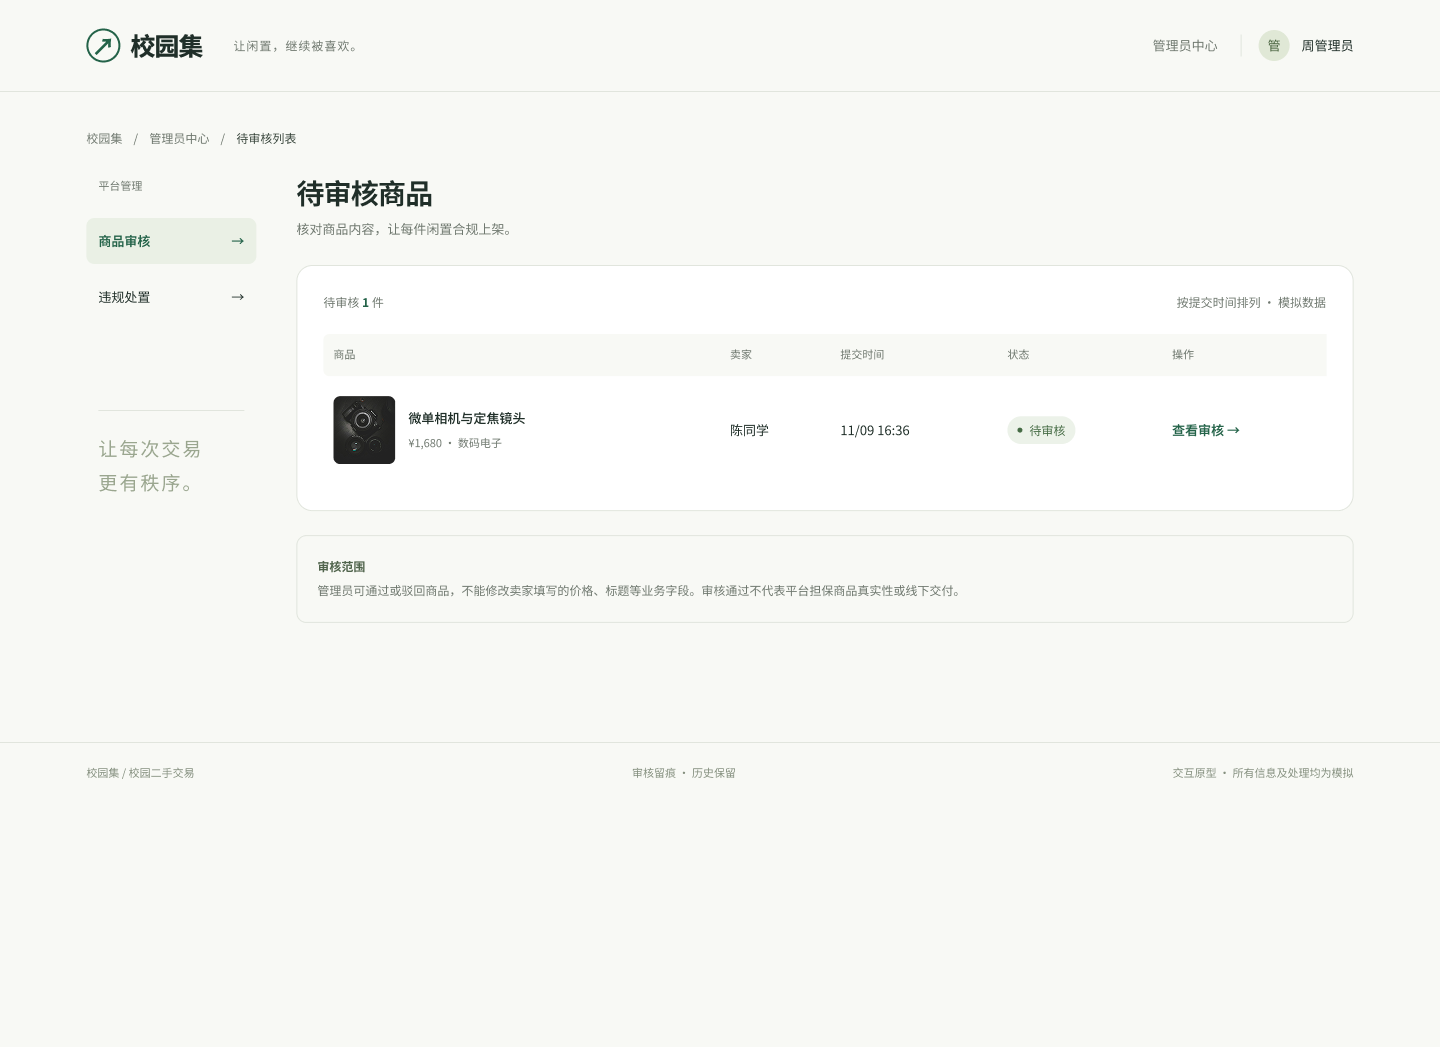
\includegraphics[width=\linewidth,height=0.60\textheight,keepaspectratio]{Report/assets/ui-14.png}
\caption{管理员待审核商品列表}
\end{figure}


审核通过后商品进入已发布；审核驳回须说明原因并退回草稿。
管理员不能借审核入口代改卖家商品字段，审核也不构成对商品真实性或线下交付的担保。


\clearpage

\subsubsection{审核详情与历史记录}
详情保持卖家内容只读，管理员可通过或填写原因后驳回。
历史按次追加并关联被审核版本，重新送审不覆盖之前驳回理由。




\begin{figure}[H]
\centering
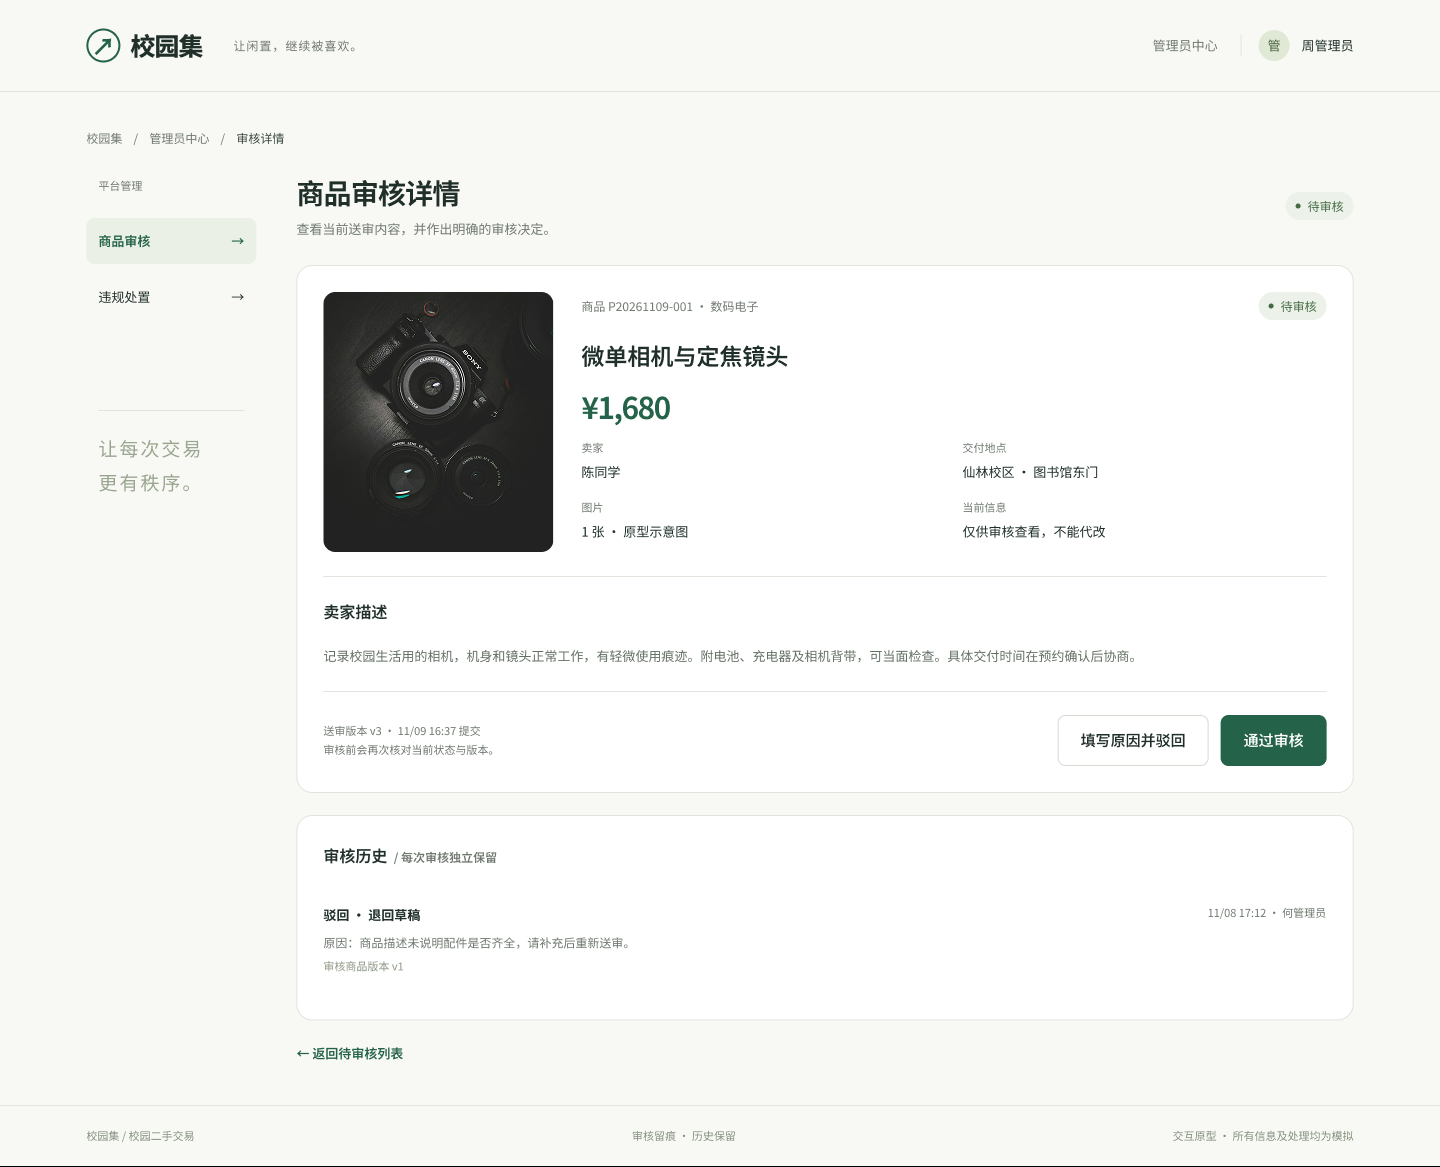
\includegraphics[width=\linewidth,height=0.68\textheight,keepaspectratio]{Report/assets/ui-15.png}
\caption{待审核详情：只读商品信息、通过与驳回入口}
\end{figure}


\clearpage

\subsubsection{审核驳回结果}
驳回完成后商品回草稿，详情展示处理原因和历史记录，两种审核按钮均关闭。
现有截图可证明原型包含驳回展示；审核通过后的已发布结果还没有独立导出图，不把“存在通过按钮”等同于该结果截图已齐备。



\begin{figure}[H]
\centering
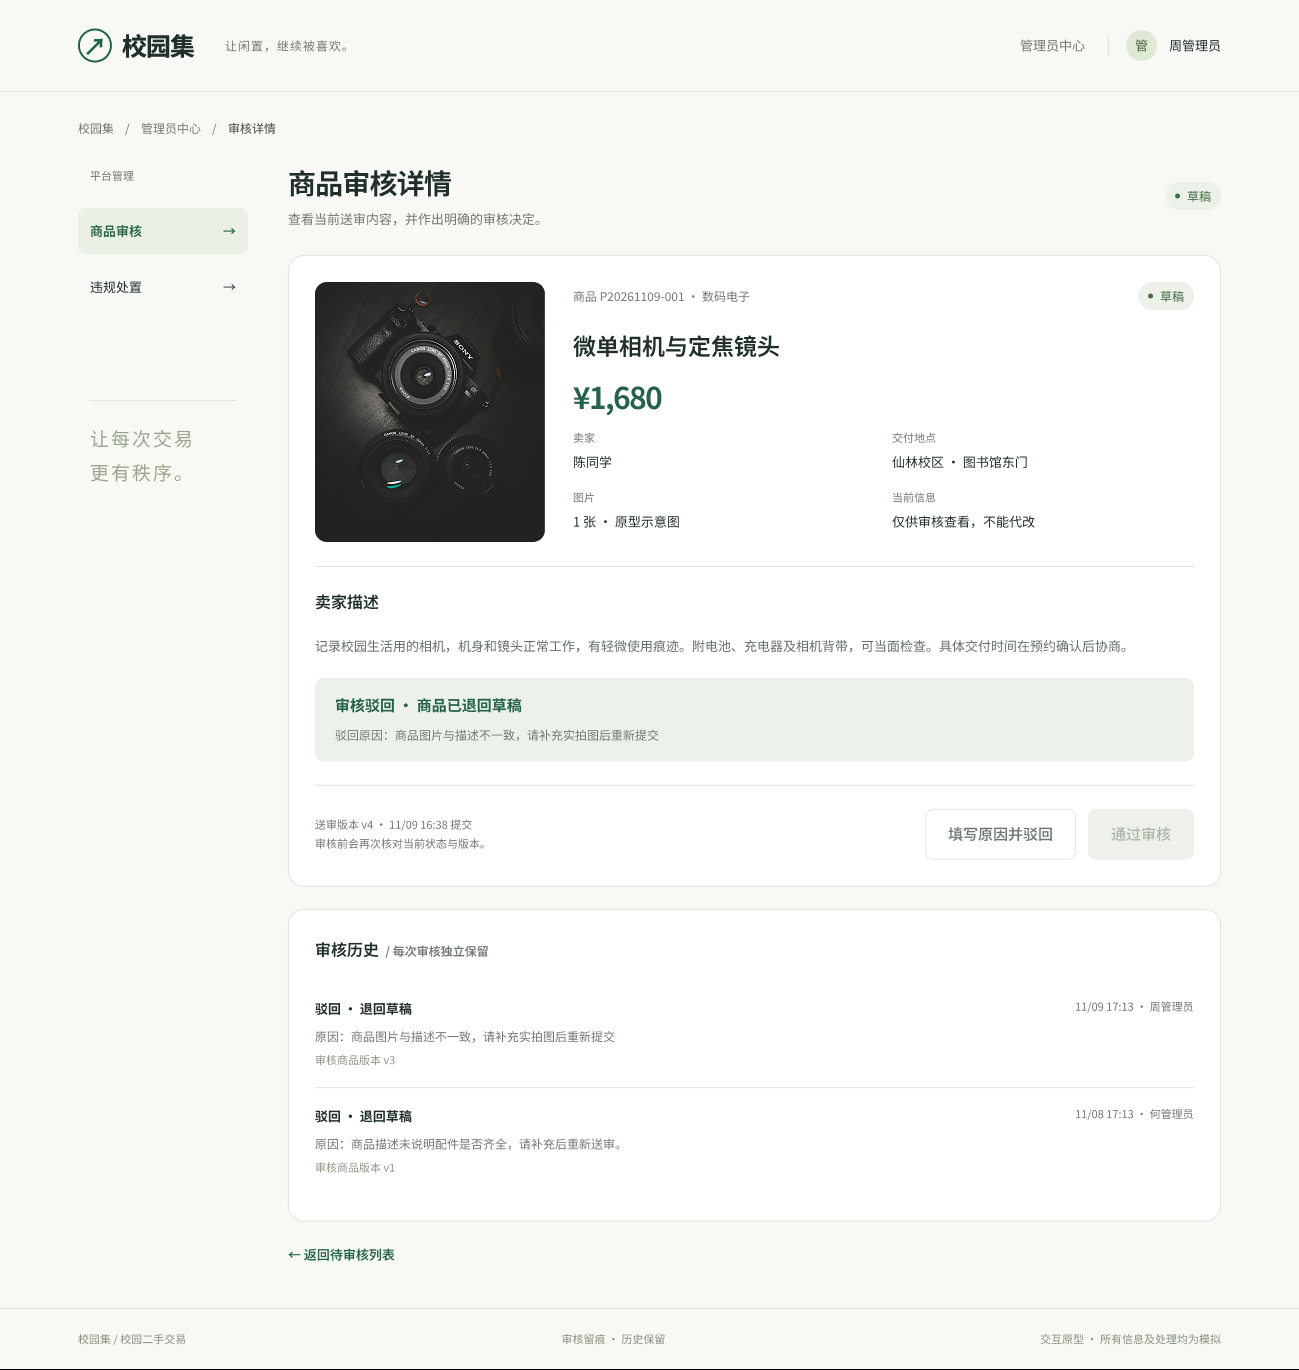
\includegraphics[width=\linewidth,height=0.69\textheight,keepaspectratio]{Report/assets/ui-16.png}
\caption{审核驳回：退回草稿与追加审核历史}
\end{figure}


\clearpage

\subsection{违规处置：原因与影响范围}
操作前展示商品当前状态、关联有效预约及价格快照，说明下架将同步终止有效预约。
违规理由必填，处理人和原因须留痕；该路径不以买卖双方同意为前提。




\begin{figure}[H]
\centering
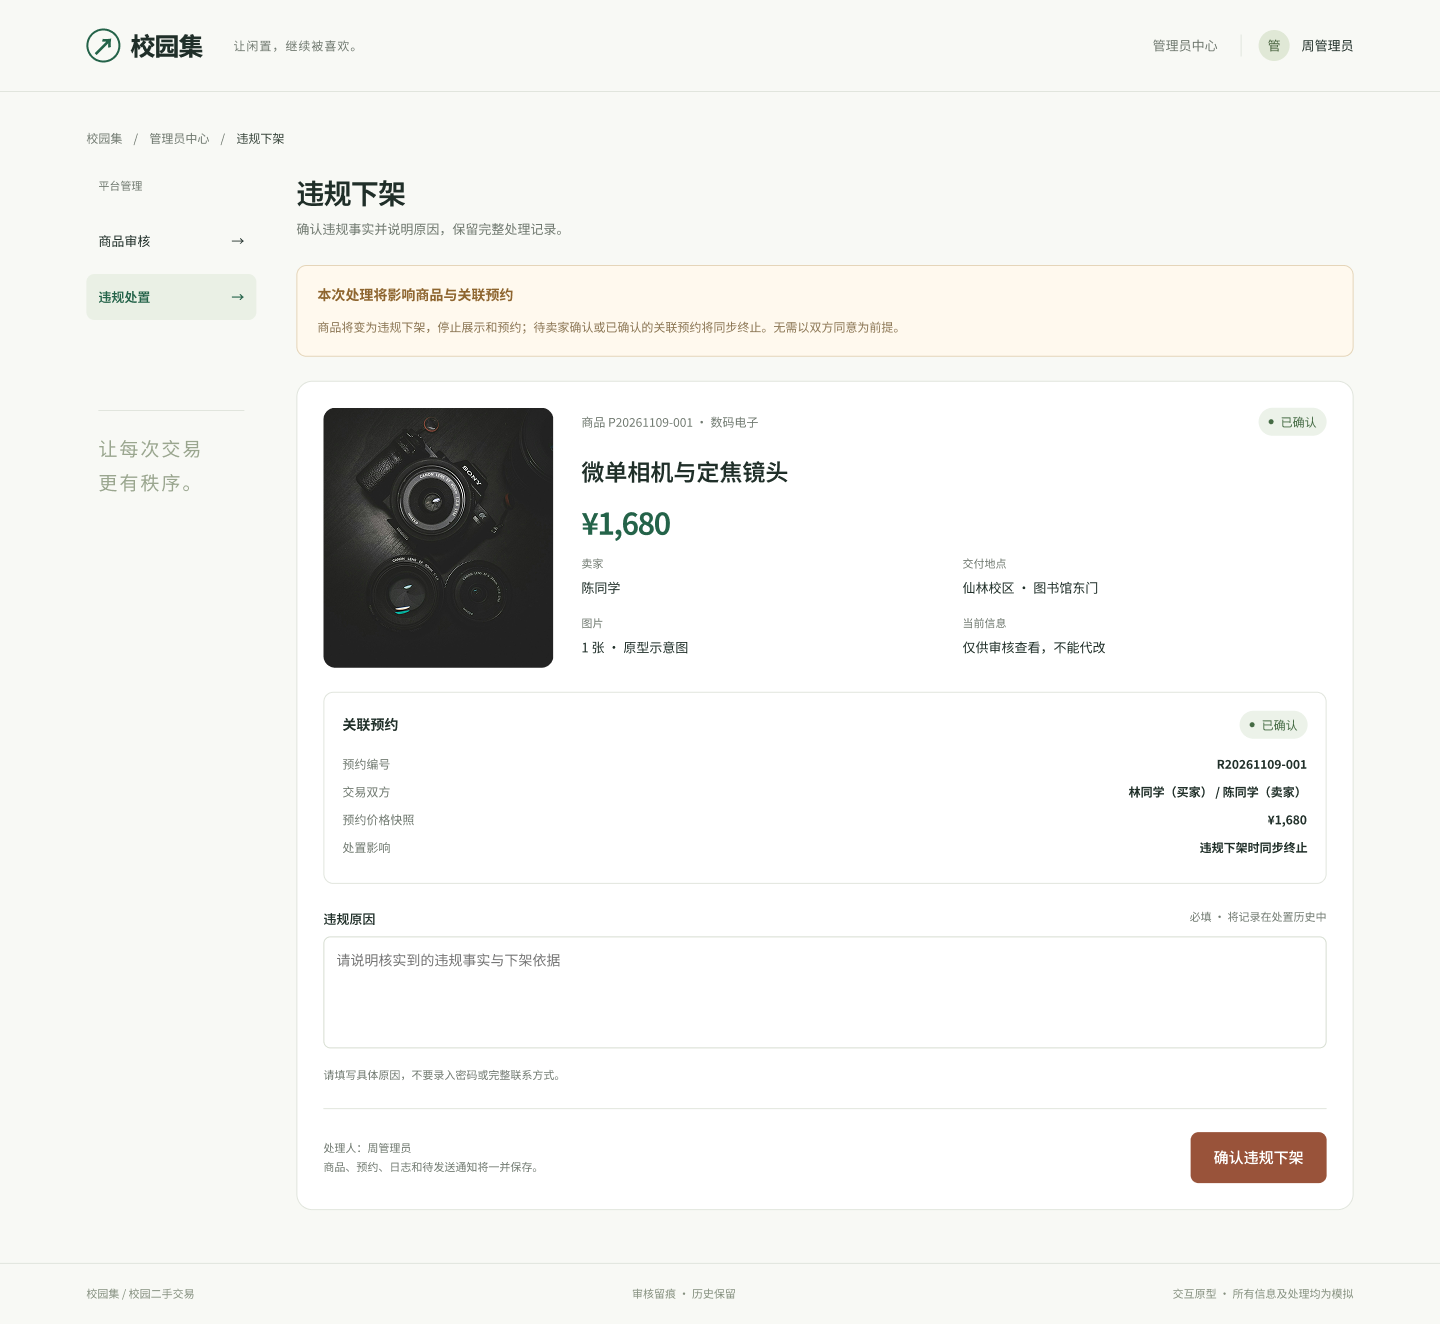
\includegraphics[width=\linewidth,height=0.68\textheight,keepaspectratio]{Report/assets/ui-17.png}
\caption{违规下架表单：关联预约与必填违规原因}
\end{figure}


\clearpage

\subsubsection{违规处置结果}
结果将商品和预约的前后状态并列展示：商品已确认转违规下架，关联预约已确认转已终止。
同时展示历史快照保留、日志记录及待发送通知，避免把“已登记通知”误写成实际投递成功。
对于已完成交易，应走保持完成状态、追加记录和隐藏的例外流程；该例外尚缺独立结果截图。



\begin{figure}[H]
\centering
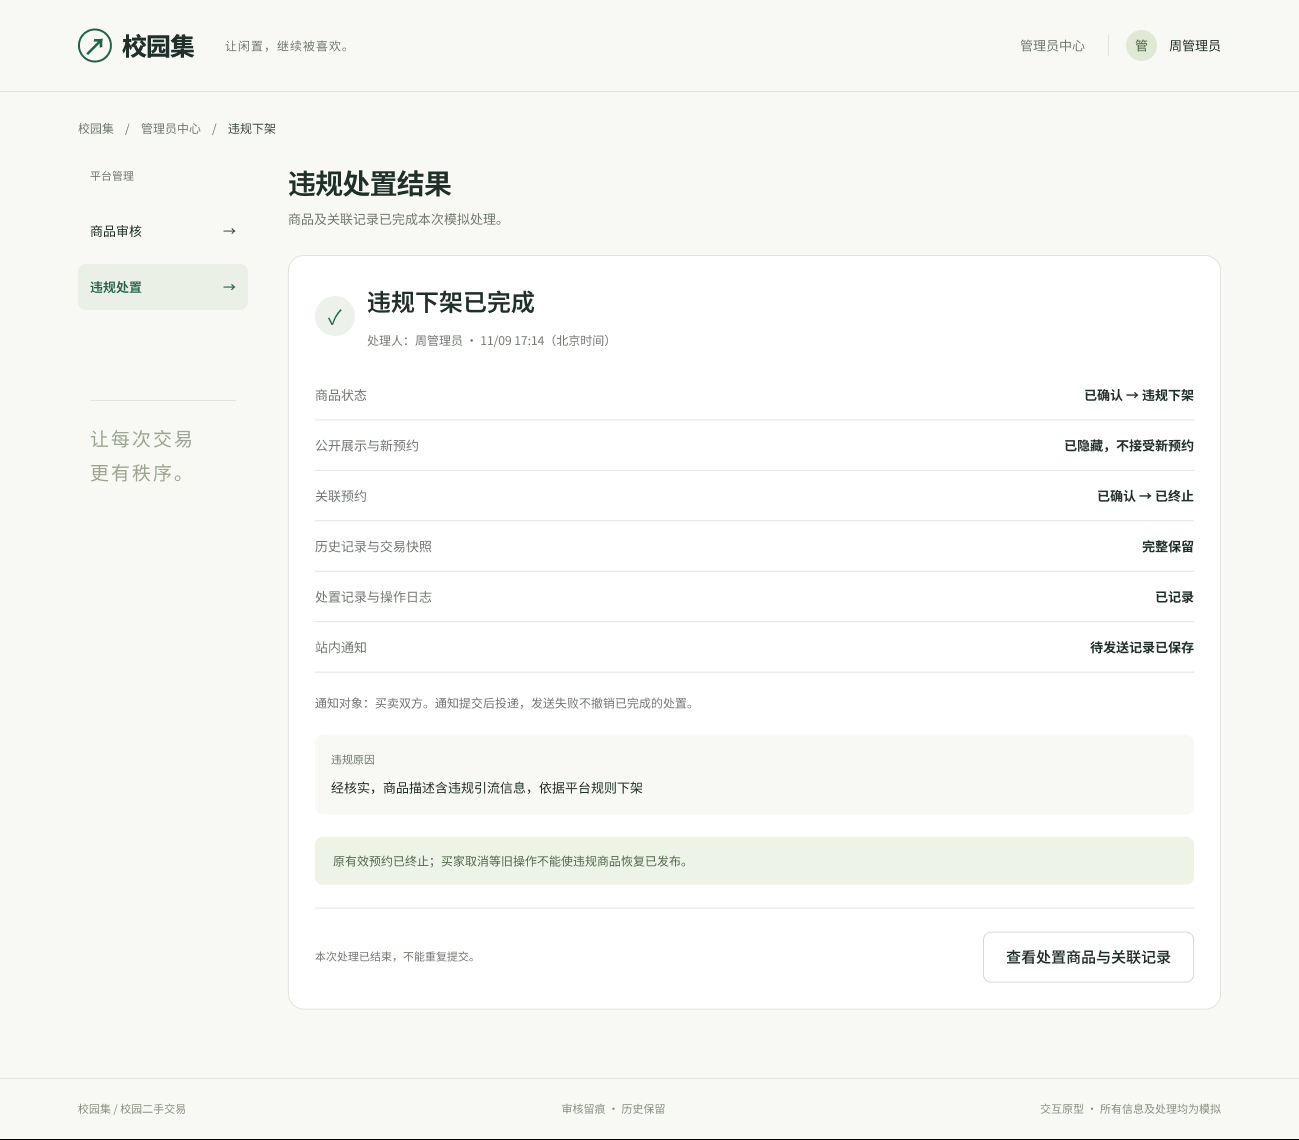
\includegraphics[width=\linewidth,height=0.68\textheight,keepaspectratio]{Report/assets/ui-18.png}
\caption{违规处置成功：商品限制、有效预约终止与待发送通知}
\end{figure}


\clearpage

\subsection{预约进度与终止申请}
买家在“我的预约”中按状态查看可执行操作：待确认可取消，已确认可确认收货或申请终止，已完成只保留历史。
终止申请记录关联预约与申请理由，同一预约同一时刻最多一条待处理申请。




\begin{figure}[H]
\centering
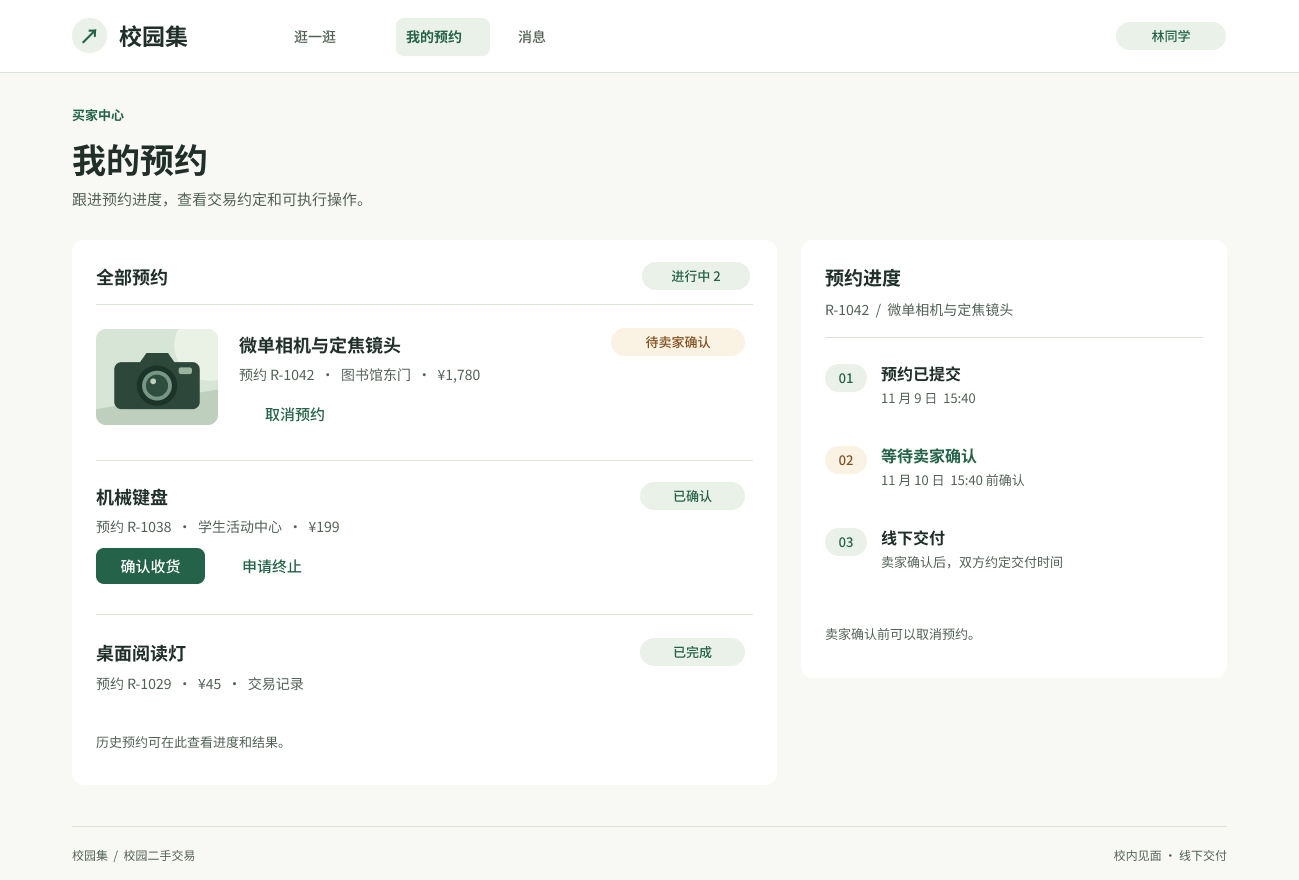
\includegraphics[width=\linewidth,height=0.34\textheight,keepaspectratio]{Report/assets/ui-19.png}
\caption{我的预约：按状态区分操作入口}
\end{figure}



\begin{figure}[H]
\centering
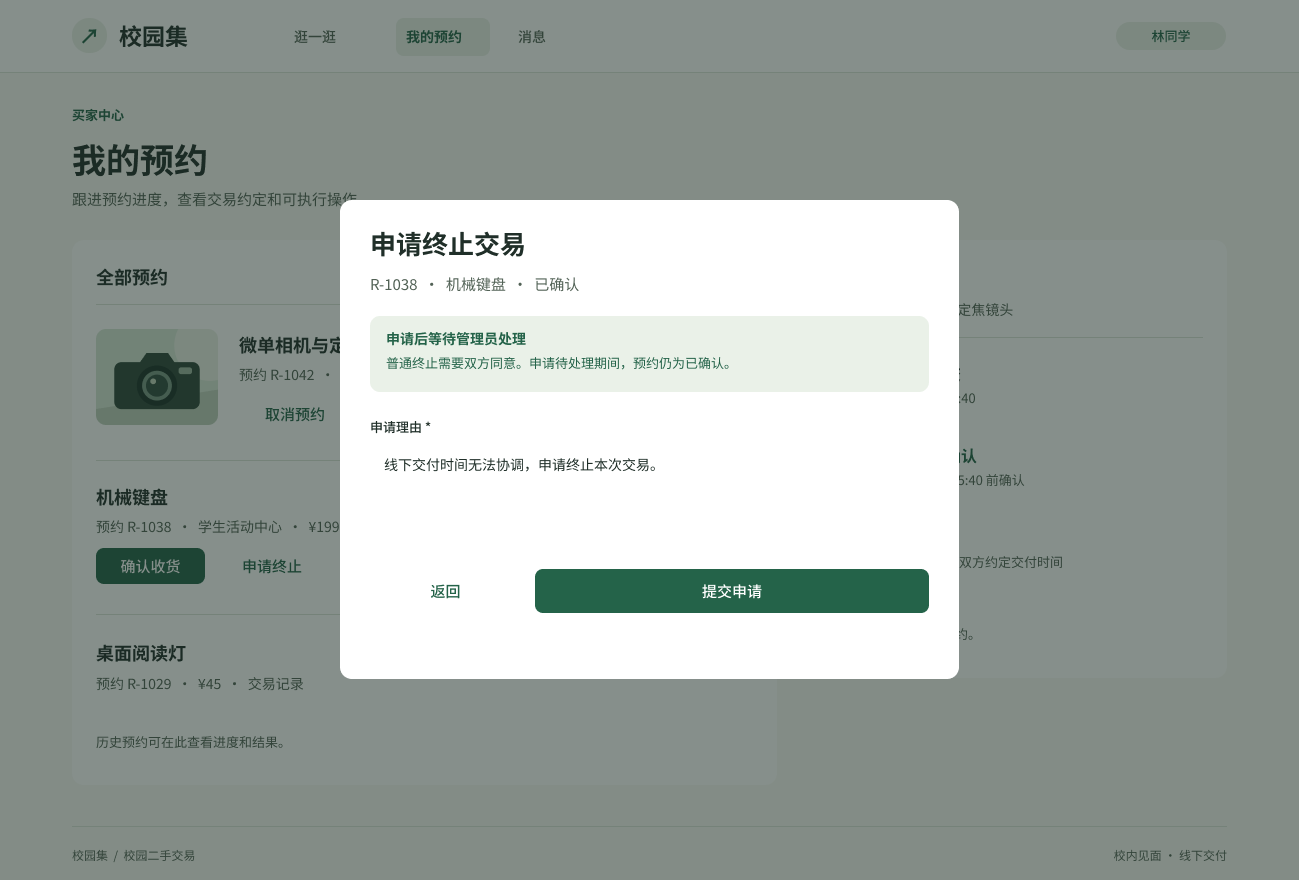
\includegraphics[width=\linewidth,height=0.34\textheight,keepaspectratio]{Report/assets/ui-20.png}
\caption{参与者申请终止交易}
\end{figure}


\clearpage

\subsubsection{管理员核实普通终止}
普通终止的管理员界面记录买家意见、卖家意见与处理原因。
只有核实双方同意并且预约仍已确认时才能批准；批准后预约已终止、商品普通已下架，驳回则维持已确认。
若买家已先确认完成，原终止申请应关闭，管理员不得再据旧页面终止。




\begin{figure}[H]
\centering
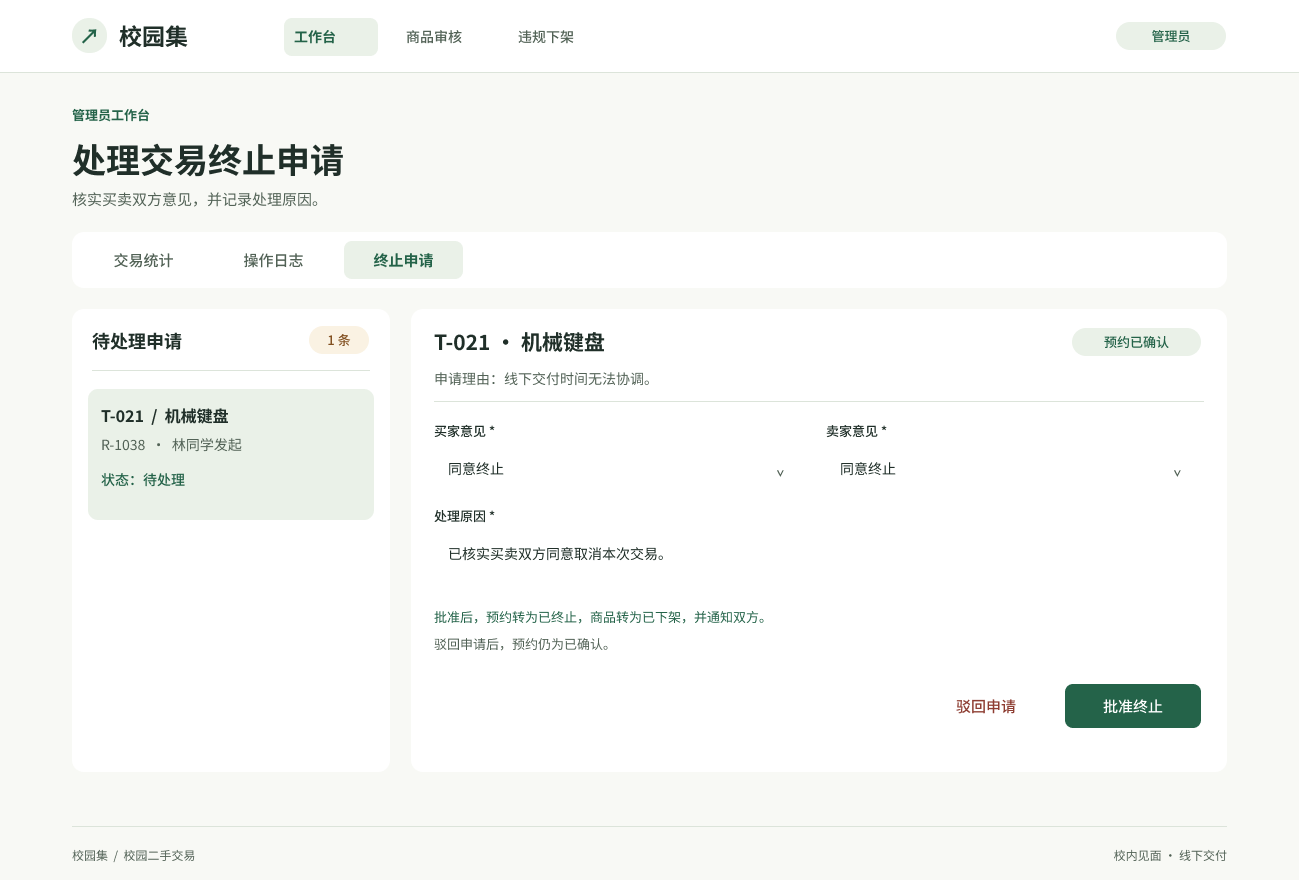
\includegraphics[width=\linewidth,height=0.58\textheight,keepaspectratio]{Report/assets/ui-21.png}
\caption{管理员处理普通终止申请：双方意见与处理原因}
\end{figure}


此画面展示的是普通终止的审批输入，不能与无需双方同意的违规终止混为同一个流程。
原型仅展示模拟数据，不声称系统已经验证线下双方意见的真实性。


\clearpage

\subsection{通知：站内消息}
消息按接收人展示预约提交、卖家确认、交易终止与违规下架等事件，区分已读和未读，提供已读操作入口。
消息可关联商品或预约，但不能让无关用户通过消息编号越权读取联系方式。




\begin{figure}[H]
\centering
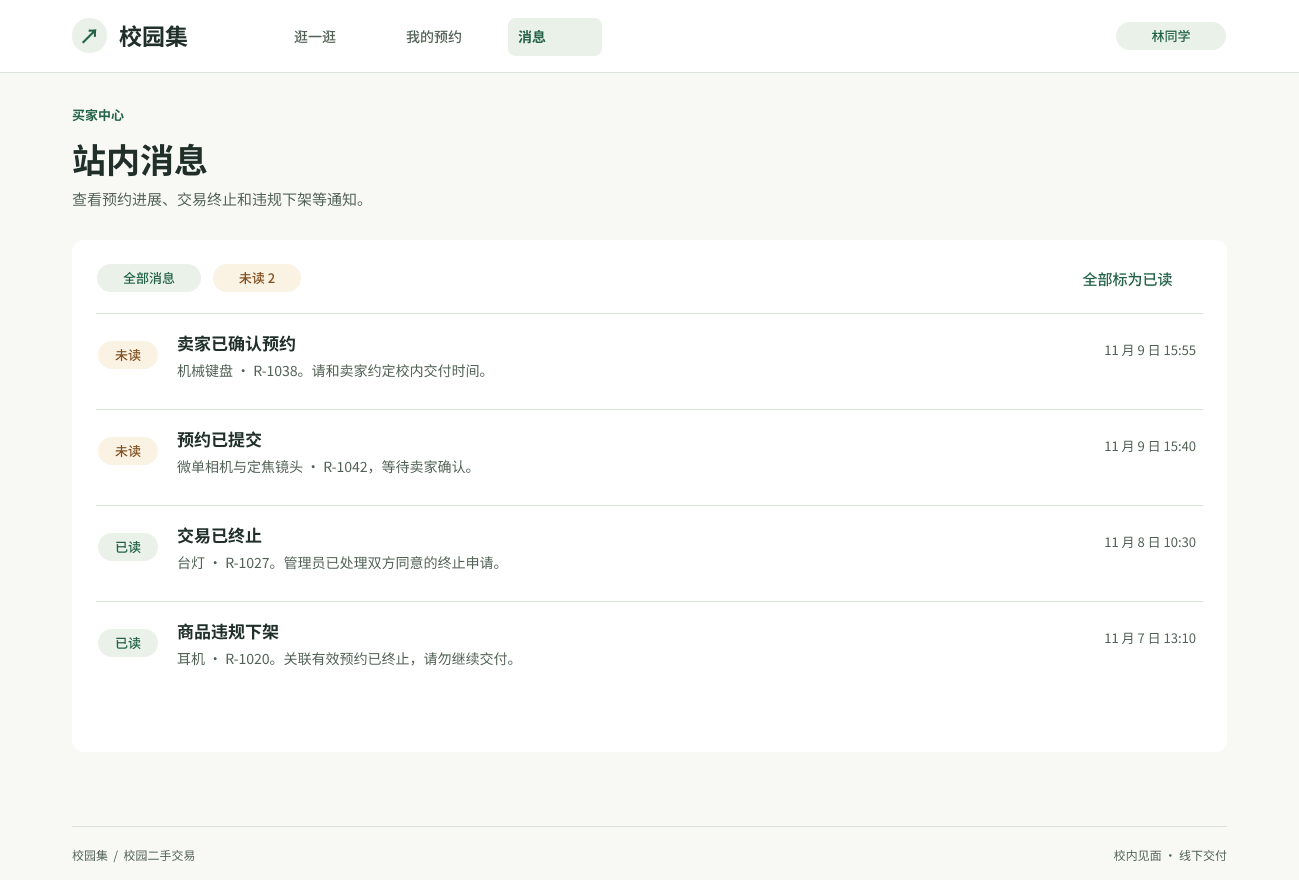
\includegraphics[width=\linewidth,height=0.59\textheight,keepaspectratio]{Report/assets/ui-22.png}
\caption{站内消息：业务关联、已读与未读状态}
\end{figure}


待发送记录与关键业务一起落库，实际投递在提交后执行。
本地原型中的消息是预置演示内容；没有发送后台，也不证明通知已在真实事务中持久保存。


\clearpage

\subsection{分类与交易统计}
统计提供日期范围、分类、卖家筛选及商品数量、已完成笔数、成交金额汇总。
商品数量按创建时间和当前状态，完成交易按完成时间统计；金额采用预约价格快照，不称为平台收入。
管理员看全站，普通用户必须加本人数据范围限制。




\begin{figure}[H]
\centering
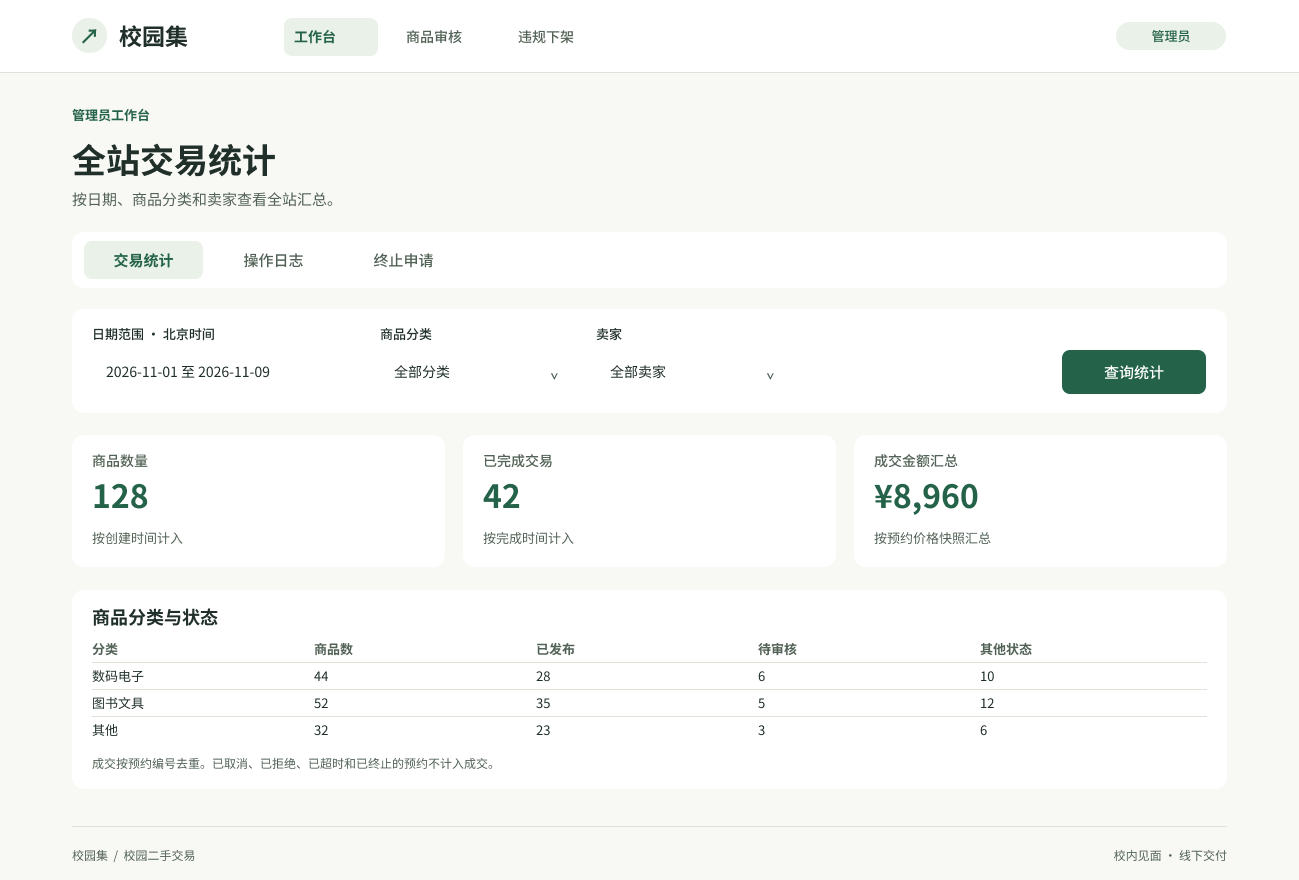
\includegraphics[width=\linewidth,height=0.59\textheight,keepaspectratio]{Report/assets/ui-23.png}
\caption{分类与交易统计：日期筛选、分组与快照金额}
\end{figure}


日期口径采用北京时间，区间从起始日零点包含至结束日期次日零点不包含。
完成交易按预约唯一编号去重，取消、拒绝、超时和终止不计入成交。截图中的128件、42笔及8960元均为模拟值。


\clearpage

\subsection{操作日志}
管理员按时间、操作者、对象编号、操作类型和结果组合查询日志。
日志显示请求标识、对象、前后状态和结果原因，只读且不开放改写、删除入口。




\begin{figure}[H]
\centering
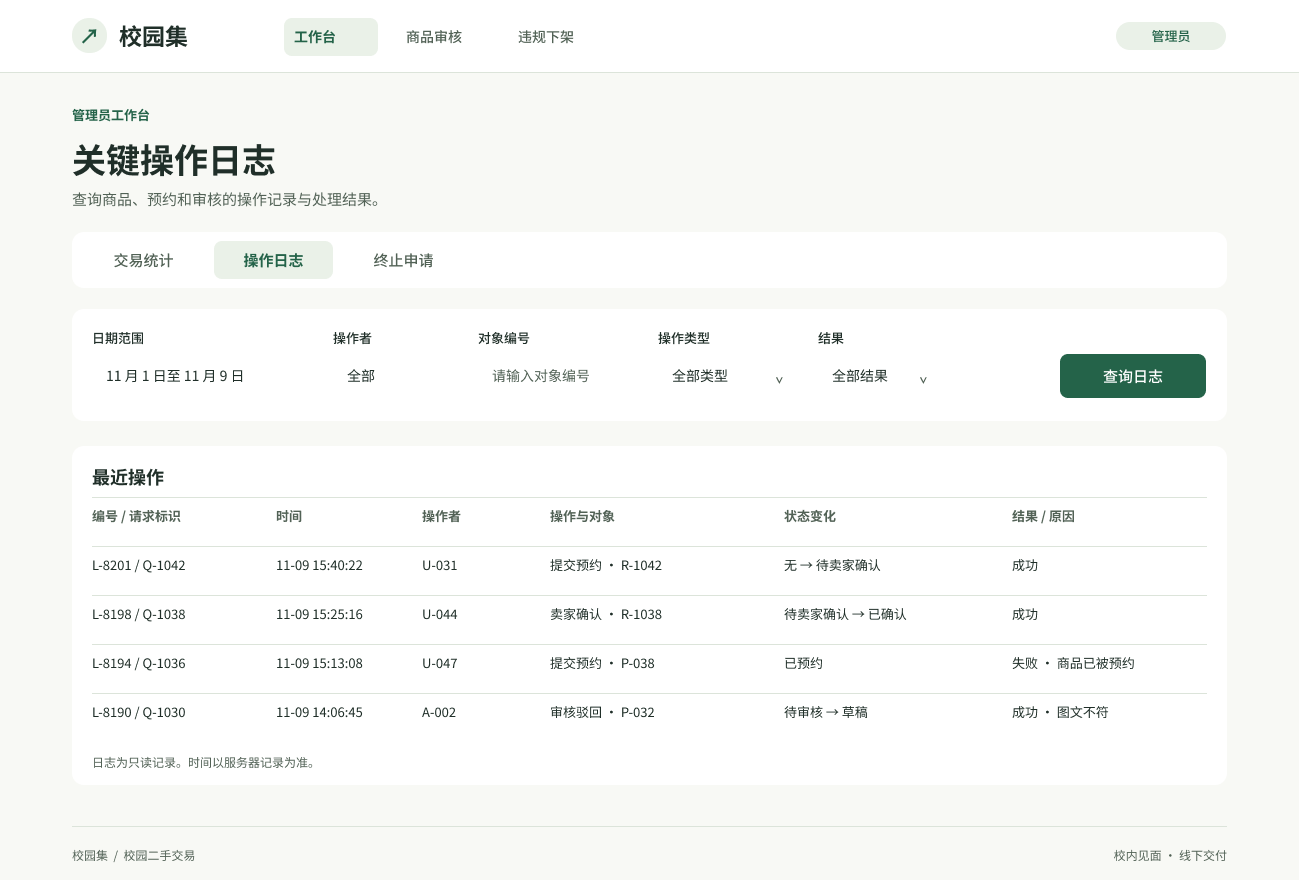
\includegraphics[width=\linewidth,height=0.59\textheight,keepaspectratio]{Report/assets/ui-24.png}
\caption{关键操作日志：组合查询与只读审计记录}
\end{figure}


成功日志与关键业务变更共同提交，失败或越权操作也要留痕。
日志不得包含密码、密码哈希或完整联系方式；保存至少180天，课程结束前不清理。
静态表格仅展示字段与反馈设计，不代表已实现不可篡改存储。


\clearpage

\section{大模型的使用}
\subsection{使用记录}
本次使用 ChatGPT/Codex 生成 UML 初稿和网页原型，并协助检查规则、整理材料和排版。主要使用情况如下。

\begingroup
\fontsize{9.5}{13}\selectfont
\renewcommand{\arraystretch}{1.15}
\begin{longtable}{@{}p{8mm}p{29mm}p{43mm}p{65mm}@{}}
\caption{大模型使用记录}\\
\toprule 序号 & 使用场景 & 生成结果 & 检查与修改\\\midrule\endfirsthead
\toprule 序号 & 使用场景 & 生成结果 & 检查与修改\\\midrule\endhead
1 & 绘制UML图 & 组件图、类图、状态图和序列图 & 核对模块依赖、关联和状态流转，补充重复请求及并发处理，调整长图布局。\\
2 & 设计UI界面 & 买家、卖家、管理员及补充界面的静态原型 & 统一界面样式，补充价格变化、原因必填、超时禁操作等反馈。\\
3 & Figma捕获 & 网页捕获步骤与界面截图 & 检查截图是否完整，确认画面状态；可编辑图层仍需在Figma中核对。\\
4 & 整理报告 & 材料清单、LaTeX源文件及PDF & 检查缺项，调整封面、字体和分页，删除重复说明。\\\bottomrule
\end{longtable}
\endgroup

\subsection{使用体会}
大模型能较快生成图和界面的初稿，省去不少重复工作。保留源码后，也方便继续调整。

但初稿不能直接当作最终结果。例如，商品可以有多条历史预约，“最多一条有效预约”需要另写约束；已完成交易发生违规时，也不能改成已终止。这些细节仍要逐条对照需求检查。

排版同样需要检查。序列图曾因过长被裁切，拆成两段后才方便阅读。网页上显示“成功”，也不代表后端已经实现事务和并发控制。

这次使用下来，大模型适合先给出一个能修改的版本。是否符合业务规则、哪里需要补充，仍要结合具体场景判断。
\end{document}
